% Options for packages loaded elsewhere
\PassOptionsToPackage{unicode}{hyperref}
\PassOptionsToPackage{hyphens}{url}
\documentclass[
  11pt,
]{article}
\usepackage{xcolor}
\usepackage[margin=1in]{geometry}
\usepackage{amsmath,amssymb}
\setcounter{secnumdepth}{5}
\usepackage{iftex}
\ifPDFTeX
  \usepackage[T1]{fontenc}
  \usepackage[utf8]{inputenc}
  \usepackage{textcomp} % provide euro and other symbols
\else % if luatex or xetex
  \usepackage{unicode-math} % this also loads fontspec
  \defaultfontfeatures{Scale=MatchLowercase}
  \defaultfontfeatures[\rmfamily]{Ligatures=TeX,Scale=1}
\fi
\usepackage{lmodern}
\ifPDFTeX\else
  % xetex/luatex font selection
\fi
% Use upquote if available, for straight quotes in verbatim environments
\IfFileExists{upquote.sty}{\usepackage{upquote}}{}
\IfFileExists{microtype.sty}{% use microtype if available
  \usepackage[]{microtype}
  \UseMicrotypeSet[protrusion]{basicmath} % disable protrusion for tt fonts
}{}
\makeatletter
\@ifundefined{KOMAClassName}{% if non-KOMA class
  \IfFileExists{parskip.sty}{%
    \usepackage{parskip}
  }{% else
    \setlength{\parindent}{0pt}
    \setlength{\parskip}{6pt plus 2pt minus 1pt}}
}{% if KOMA class
  \KOMAoptions{parskip=half}}
\makeatother
\usepackage{color}
\usepackage{fancyvrb}
\newcommand{\VerbBar}{|}
\newcommand{\VERB}{\Verb[commandchars=\\\{\}]}
\DefineVerbatimEnvironment{Highlighting}{Verbatim}{commandchars=\\\{\}}
% Add ',fontsize=\small' for more characters per line
\usepackage{framed}
\definecolor{shadecolor}{RGB}{248,248,248}
\newenvironment{Shaded}{\begin{snugshade}}{\end{snugshade}}
\newcommand{\AlertTok}[1]{\textcolor[rgb]{0.94,0.16,0.16}{#1}}
\newcommand{\AnnotationTok}[1]{\textcolor[rgb]{0.56,0.35,0.01}{\textbf{\textit{#1}}}}
\newcommand{\AttributeTok}[1]{\textcolor[rgb]{0.13,0.29,0.53}{#1}}
\newcommand{\BaseNTok}[1]{\textcolor[rgb]{0.00,0.00,0.81}{#1}}
\newcommand{\BuiltInTok}[1]{#1}
\newcommand{\CharTok}[1]{\textcolor[rgb]{0.31,0.60,0.02}{#1}}
\newcommand{\CommentTok}[1]{\textcolor[rgb]{0.56,0.35,0.01}{\textit{#1}}}
\newcommand{\CommentVarTok}[1]{\textcolor[rgb]{0.56,0.35,0.01}{\textbf{\textit{#1}}}}
\newcommand{\ConstantTok}[1]{\textcolor[rgb]{0.56,0.35,0.01}{#1}}
\newcommand{\ControlFlowTok}[1]{\textcolor[rgb]{0.13,0.29,0.53}{\textbf{#1}}}
\newcommand{\DataTypeTok}[1]{\textcolor[rgb]{0.13,0.29,0.53}{#1}}
\newcommand{\DecValTok}[1]{\textcolor[rgb]{0.00,0.00,0.81}{#1}}
\newcommand{\DocumentationTok}[1]{\textcolor[rgb]{0.56,0.35,0.01}{\textbf{\textit{#1}}}}
\newcommand{\ErrorTok}[1]{\textcolor[rgb]{0.64,0.00,0.00}{\textbf{#1}}}
\newcommand{\ExtensionTok}[1]{#1}
\newcommand{\FloatTok}[1]{\textcolor[rgb]{0.00,0.00,0.81}{#1}}
\newcommand{\FunctionTok}[1]{\textcolor[rgb]{0.13,0.29,0.53}{\textbf{#1}}}
\newcommand{\ImportTok}[1]{#1}
\newcommand{\InformationTok}[1]{\textcolor[rgb]{0.56,0.35,0.01}{\textbf{\textit{#1}}}}
\newcommand{\KeywordTok}[1]{\textcolor[rgb]{0.13,0.29,0.53}{\textbf{#1}}}
\newcommand{\NormalTok}[1]{#1}
\newcommand{\OperatorTok}[1]{\textcolor[rgb]{0.81,0.36,0.00}{\textbf{#1}}}
\newcommand{\OtherTok}[1]{\textcolor[rgb]{0.56,0.35,0.01}{#1}}
\newcommand{\PreprocessorTok}[1]{\textcolor[rgb]{0.56,0.35,0.01}{\textit{#1}}}
\newcommand{\RegionMarkerTok}[1]{#1}
\newcommand{\SpecialCharTok}[1]{\textcolor[rgb]{0.81,0.36,0.00}{\textbf{#1}}}
\newcommand{\SpecialStringTok}[1]{\textcolor[rgb]{0.31,0.60,0.02}{#1}}
\newcommand{\StringTok}[1]{\textcolor[rgb]{0.31,0.60,0.02}{#1}}
\newcommand{\VariableTok}[1]{\textcolor[rgb]{0.00,0.00,0.00}{#1}}
\newcommand{\VerbatimStringTok}[1]{\textcolor[rgb]{0.31,0.60,0.02}{#1}}
\newcommand{\WarningTok}[1]{\textcolor[rgb]{0.56,0.35,0.01}{\textbf{\textit{#1}}}}
\usepackage{longtable,booktabs,array}
\newcounter{none} % for unnumbered tables
\usepackage{calc} % for calculating minipage widths
% Correct order of tables after \paragraph or \subparagraph
\usepackage{etoolbox}
\makeatletter
\patchcmd\longtable{\par}{\if@noskipsec\mbox{}\fi\par}{}{}
\makeatother
% Allow footnotes in longtable head/foot
\IfFileExists{footnotehyper.sty}{\usepackage{footnotehyper}}{\usepackage{footnote}}
\makesavenoteenv{longtable}
\usepackage{graphicx}
\makeatletter
\newsavebox\pandoc@box
\newcommand*\pandocbounded[1]{% scales image to fit in text height/width
  \sbox\pandoc@box{#1}%
  \Gscale@div\@tempa{\textheight}{\dimexpr\ht\pandoc@box+\dp\pandoc@box\relax}%
  \Gscale@div\@tempb{\linewidth}{\wd\pandoc@box}%
  \ifdim\@tempb\p@<\@tempa\p@\let\@tempa\@tempb\fi% select the smaller of both
  \ifdim\@tempa\p@<\p@\scalebox{\@tempa}{\usebox\pandoc@box}%
  \else\usebox{\pandoc@box}%
  \fi%
}
% Set default figure placement to htbp
\def\fps@figure{htbp}
\makeatother
\setlength{\emergencystretch}{3em} % prevent overfull lines
\providecommand{\tightlist}{%
  \setlength{\itemsep}{0pt}\setlength{\parskip}{0pt}}
\usepackage{fvextra}
\DefineVerbatimEnvironment{Highlighting}{Verbatim}{breaklines,breakanywhere,commandchars=\\\{\}}
\DefineVerbatimEnvironment{verbatim}{Verbatim}{breaklines,breakanywhere}
\usepackage{float}
\usepackage{longtable}
\usepackage{booktabs}
\usepackage{longtable}
\usepackage{array}
\usepackage{multirow}
\usepackage{wrapfig}
\usepackage{float}
\usepackage{colortbl}
\usepackage{pdflscape}
\usepackage{tabularx}
\usepackage{xltabular}
\usepackage{threeparttable}
\usepackage{threeparttablex}
\usepackage[normalem]{ulem}
\usepackage{makecell}
\usepackage{xcolor}
\usepackage{bookmark}
\IfFileExists{xurl.sty}{\usepackage{xurl}}{} % add URL line breaks if available
\urlstyle{same}
\hypersetup{
  pdftitle={ASESII 24A02 Final Project},
  hidelinks,
  pdfcreator={LaTeX via pandoc}}

\title{ASESII 24A02 Final Project}
\usepackage{etoolbox}
\makeatletter
\providecommand{\subtitle}[1]{% add subtitle to \maketitle
  \apptocmd{\@title}{\par {\large #1 \par}}{}{}
}
\makeatother
\subtitle{Predict noise level generated by NACA airfoil blade sections}
\author{Group 02\\
Nguyen Thi Yen Nhi (24125071)\\
Nguyen Khang Thinh (24125104)\\
Nguyen Van Tinh (24125106)\\
Nguyen Le Quoc Huy (24125100)}
\date{2026-08-23}

\begin{document}
\maketitle

{
\setcounter{tocdepth}{2}
\tableofcontents
}
\section*{Authorship and contribution
statement}\label{authorship-and-contribution-statement}
\addcontentsline{toc}{section}{Authorship and contribution statement}

  \begingroup
  \renewcommand{\arraystretch}{1.3}
  \begin{tabular}{p{0.25\linewidth} p{0.09\linewidth} p{0.57\linewidth}}
  \hline
  Student & ID & Main contributions  \\
  \hline
  Nguyen Thi Yen Nhi & 24125071 &
  Target and predictors, split and preprocessing plan, and data exploration  \\
  \hline
  Nguyen Khang Thinh & 24125104 &
  Dataset selection, research questions, hypotheses, and descriptive statistics for the experimental design \\
  \hline
  Nguyen Van Tinh & 24125106 &
  OLS, Ridge, and Lasso regression, including model fitting, regularization, coefficient analysis, and model comparison \\
  \hline
  Nguyen Le Quoc Huy & 24125100 &
  ANOVA/factorial design analysis, post-hoc analysis, and conclusion and evaluation \\
  \hline
  \end{tabular}
  \endgroup

\section*{Abstract}\label{abstract}
\addcontentsline{toc}{section}{Abstract}

This study investigates the prediction of sound pressure levels
generated by NACA 0012 airfoil blade sections using five aerodynamic and
geometric predictors. The dataset contains 1,503 wind-tunnel
observations with no missing values, duplicate rows, or physically
invalid measurements. Exploratory analysis revealed weak individual
predictor-response relationships and moderate correlation between attack
angle and suction-side displacement thickness, while the
frequency-response relationship showed evidence of nonlinearity.

We compared Ordinary Least Squares (OLS), Ridge, and Lasso regression
using an 80/20 train-test split and five-fold cross-validation.
Predictors were standardized using training-set statistics only to
prevent data leakage. OLS achieved a cross-validation MSE of 23.03,
while Ridge and Lasso produced similar predictive errors. However, Ridge
substantially improved numerical conditioning, reducing the condition
number from 12.30 for OLS to 5.34 at its optimal penalty. Lasso did not
eliminate any of the five original predictors at either tuning rule.

A perturbation experiment introduced a near-duplicate predictor highly
correlated with frequency (r=0.995) to evaluate model stability under
stronger multicollinearity. Ridge maintained stable predictive
performance by redistributing coefficients across correlated predictors,
whereas Lasso demonstrated variable-selection behavior under the more
conservative 1SE rule.

Overall, the results show that regularization provides greater numerical
stability without sacrificing substantial predictive accuracy, with
Ridge offering the most consistent response to multicollinearity in this
dataset.

\section{Prediction design and leakage
control}\label{prediction-design-and-leakage-control}

\subsection{Target and predictors}\label{target-and-predictors}

\begin{Shaded}
\begin{Highlighting}[]
\NormalTok{data }\OtherTok{\textless{}{-}} \FunctionTok{read.table}\NormalTok{(}\StringTok{"data/airfoil\_self\_noise.dat"}\NormalTok{, }\AttributeTok{header =} \ConstantTok{FALSE}\NormalTok{)}
\FunctionTok{colnames}\NormalTok{(data) }\OtherTok{\textless{}{-}} \FunctionTok{c}\NormalTok{(}\StringTok{"frequency"}\NormalTok{, }\StringTok{"attack\_angle"}\NormalTok{, }\StringTok{"chord\_length"}\NormalTok{, }\StringTok{"free\_stream\_velocity"}\NormalTok{, }\StringTok{"suction\_side\_displacement\_thickness"}\NormalTok{, }\StringTok{"scaled\_sound\_pressure"}\NormalTok{)}

\CommentTok{\# Always (re)written from the .dat source so the cached CSV can never drift}
\CommentTok{\# from the column{-}naming convention fixed above.}
\FunctionTok{write.csv}\NormalTok{(}
\NormalTok{  data,}
  \StringTok{"data/airfoil\_self\_noise.csv"}\NormalTok{,}
  \AttributeTok{row.names =} \ConstantTok{FALSE}
\NormalTok{)}

\FunctionTok{str}\NormalTok{(data)}
\end{Highlighting}
\end{Shaded}

\begin{verbatim}
## 'data.frame':    1503 obs. of  6 variables:
##  $ frequency                          : int  800 1000 1250 1600 2000 2500 3150 4000 5000 6300 ...
##  $ attack_angle                       : num  0 0 0 0 0 0 0 0 0 0 ...
##  $ chord_length                       : num  0.305 0.305 0.305 0.305 0.305 ...
##  $ free_stream_velocity               : num  71.3 71.3 71.3 71.3 71.3 71.3 71.3 71.3 71.3 71.3 ...
##  $ suction_side_displacement_thickness: num  0.00266 0.00266 0.00266 0.00266 0.00266 ...
##  $ scaled_sound_pressure              : num  126 125 126 128 127 ...
\end{verbatim}

\begin{Shaded}
\begin{Highlighting}[]
\NormalTok{config }\OtherTok{\textless{}{-}} \FunctionTok{list}\NormalTok{(}
  \AttributeTok{file =} \StringTok{"airfoil\_self\_noise.csv"}\NormalTok{,}
  \AttributeTok{response =} \StringTok{"scaled\_sound\_pressure"}\NormalTok{,}
  \AttributeTok{excluded =} \StringTok{"scaled\_sound\_pressure"}
\NormalTok{)}
\NormalTok{data\_raw }\OtherTok{\textless{}{-}} \FunctionTok{read.csv}\NormalTok{(}\FunctionTok{find\_exam\_data}\NormalTok{(config}\SpecialCharTok{$}\NormalTok{file), }\AttributeTok{check.names =} \ConstantTok{FALSE}\NormalTok{)}
\NormalTok{predictors }\OtherTok{\textless{}{-}} \FunctionTok{setdiff}\NormalTok{(}\FunctionTok{names}\NormalTok{(data\_raw), config}\SpecialCharTok{$}\NormalTok{excluded)}
\NormalTok{analysis\_data }\OtherTok{\textless{}{-}}\NormalTok{ data\_raw[, }\FunctionTok{c}\NormalTok{(config}\SpecialCharTok{$}\NormalTok{response, predictors), drop }\OtherTok{=} \ConstantTok{FALSE}\NormalTok{]}

\ControlFlowTok{if}\NormalTok{ (}\FunctionTok{anyNA}\NormalTok{(analysis\_data)) }\FunctionTok{stop}\NormalTok{(}\StringTok{"Declare a training{-}only missing{-}value plan."}\NormalTok{)}
\ControlFlowTok{if}\NormalTok{ (}\SpecialCharTok{!}\FunctionTok{all}\NormalTok{(}\FunctionTok{vapply}\NormalTok{(analysis\_data, is.numeric, }\FunctionTok{logical}\NormalTok{(}\DecValTok{1}\NormalTok{)))) \{}
  \FunctionTok{stop}\NormalTok{(}\StringTok{"The assigned response and predictors must be numeric."}\NormalTok{)}
\NormalTok{\}}
\end{Highlighting}
\end{Shaded}

\pandocbounded{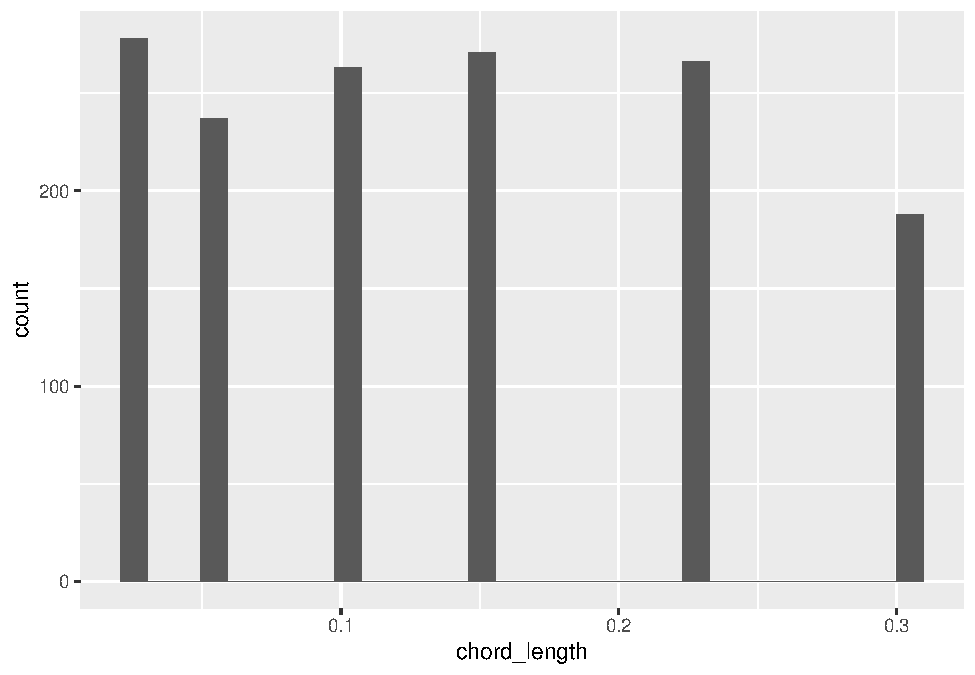
\includegraphics[keepaspectratio]{main_files/main_files/figure-latex/data-overview-1.pdf}}

\begin{longtable}[]{@{}
  >{\raggedright\arraybackslash}p{(\linewidth - 8\tabcolsep) * \real{0.5070}}
  >{\raggedright\arraybackslash}p{(\linewidth - 8\tabcolsep) * \real{0.1408}}
  >{\raggedright\arraybackslash}p{(\linewidth - 8\tabcolsep) * \real{0.1127}}
  >{\raggedleft\arraybackslash}p{(\linewidth - 8\tabcolsep) * \real{0.1268}}
  >{\raggedleft\arraybackslash}p{(\linewidth - 8\tabcolsep) * \real{0.1127}}@{}}
\caption{Response and candidate predictors, with the integrity checks
run before the split.}\tabularnewline
\toprule\noalign{}
\begin{minipage}[b]{\linewidth}\raggedright
Variable
\end{minipage} & \begin{minipage}[b]{\linewidth}\raggedright
Role
\end{minipage} & \begin{minipage}[b]{\linewidth}\raggedright
Type
\end{minipage} & \begin{minipage}[b]{\linewidth}\raggedleft
Distinct
\end{minipage} & \begin{minipage}[b]{\linewidth}\raggedleft
Missing
\end{minipage} \\
\midrule\noalign{}
\endfirsthead
\toprule\noalign{}
\begin{minipage}[b]{\linewidth}\raggedright
Variable
\end{minipage} & \begin{minipage}[b]{\linewidth}\raggedright
Role
\end{minipage} & \begin{minipage}[b]{\linewidth}\raggedright
Type
\end{minipage} & \begin{minipage}[b]{\linewidth}\raggedleft
Distinct
\end{minipage} & \begin{minipage}[b]{\linewidth}\raggedleft
Missing
\end{minipage} \\
\midrule\noalign{}
\endhead
\bottomrule\noalign{}
\endlastfoot
frequency & Predictor & integer & 21 & 0 \\
attack\_angle & Predictor & numeric & 27 & 0 \\
chord\_length & Predictor & numeric & 6 & 0 \\
free\_stream\_velocity & Predictor & numeric & 4 & 0 \\
suction\_side\_displacement\_thickness & Predictor & numeric & 105 &
0 \\
scaled\_sound\_pressure & Response & numeric & 1456 & 0 \\
\end{longtable}

\begin{longtable}[]{@{}lr@{}}
\caption{Missing-value and duplicate-row checks on the raw
data.}\tabularnewline
\toprule\noalign{}
Check & Count \\
\midrule\noalign{}
\endfirsthead
\toprule\noalign{}
Check & Count \\
\midrule\noalign{}
\endhead
\bottomrule\noalign{}
\endlastfoot
Missing values (total cells) & 0 \\
Fully duplicated rows & 0 \\
\end{longtable}

The dataset contains 1503 observations of 6 numeric variables: five
predictors recorded during NACA 0012 airfoil wind-tunnel tests and the
response \texttt{scaled\_sound\_pressure}, the scaled sound pressure
level in decibels. No missing values or duplicated rows are present
(table above), so no imputation or de-duplication is required before the
split.

The \texttt{Distinct} column in Table 1 shows that the five predictors
are not equally ``continuous'' in practice. \texttt{frequency},
\texttt{chord\_length}, and \texttt{free\_stream\_velocity} take only
21, 6, and 4 distinct values respectively - these are the fixed
1/3-octave frequency bands, airfoil chord lengths, and wind-tunnel
speeds used to design the experiment, so each behaves more like an
ordinal experimental factor than a freely varying measurement.
\texttt{attack\_angle} (27 distinct values) and
\texttt{suction\_side\_displacement\_thickness} (105 distinct values)
are closer to genuinely continuous quantities. This low cardinality on
three of the five predictors is expected to show up later as visibly
clustered histograms and boxplots (1C) rather than smooth continuous
distributions, and is a property of the experimental design rather than
a data-quality issue.

\texttt{data/data\_description.md} (the accompanying UCI variable sheet)
lists \texttt{attack\_angle} as ``Binary'', which does not match what is
observed here - the variable takes 27 distinct values between 0 and 22.2
degrees. This looks like a labelling error in the source sheet, and
\texttt{attack\_angle} is treated as continuous throughout, consistent
with the assignment brief's own description of the dataset (``angle of
attack'' as a continuous input).

\subsection{Split and preprocessing
plan}\label{split-and-preprocessing-plan}

\begin{Shaded}
\begin{Highlighting}[]
\NormalTok{split }\OtherTok{\textless{}{-}} \FunctionTok{split\_rows}\NormalTok{(}\FunctionTok{nrow}\NormalTok{(analysis\_data), }\AttributeTok{seed =}\NormalTok{ seeds}\SpecialCharTok{$}\NormalTok{split)}
\NormalTok{train\_id }\OtherTok{\textless{}{-}}\NormalTok{ split}\SpecialCharTok{$}\NormalTok{train}
\NormalTok{test\_id }\OtherTok{\textless{}{-}}\NormalTok{ split}\SpecialCharTok{$}\NormalTok{test}
\NormalTok{train\_df }\OtherTok{\textless{}{-}}\NormalTok{ analysis\_data[train\_id, ]}

\NormalTok{x\_raw }\OtherTok{\textless{}{-}} \FunctionTok{as.matrix}\NormalTok{(analysis\_data[, predictors, }\AttributeTok{drop =} \ConstantTok{FALSE}\NormalTok{])}
\NormalTok{y\_raw }\OtherTok{\textless{}{-}}\NormalTok{ analysis\_data[[config}\SpecialCharTok{$}\NormalTok{response]]}

\NormalTok{x\_prep }\OtherTok{\textless{}{-}} \FunctionTok{fit\_scaler}\NormalTok{(x\_raw[train\_id, , }\AttributeTok{drop =} \ConstantTok{FALSE}\NormalTok{])}
\NormalTok{x\_train }\OtherTok{\textless{}{-}} \FunctionTok{apply\_scaler}\NormalTok{(x\_raw[train\_id, , }\AttributeTok{drop =} \ConstantTok{FALSE}\NormalTok{], x\_prep)}
\NormalTok{x\_test }\OtherTok{\textless{}{-}} \FunctionTok{apply\_scaler}\NormalTok{(x\_raw[test\_id, , }\AttributeTok{drop =} \ConstantTok{FALSE}\NormalTok{], x\_prep)}
\NormalTok{y\_train }\OtherTok{\textless{}{-}}\NormalTok{ y\_raw[train\_id]}
\NormalTok{y\_test }\OtherTok{\textless{}{-}}\NormalTok{ y\_raw[test\_id]}

\NormalTok{foldid }\OtherTok{\textless{}{-}} \FunctionTok{make\_foldid}\NormalTok{(}\FunctionTok{nrow}\NormalTok{(x\_train), }\AttributeTok{k =} \DecValTok{5}\DataTypeTok{L}\NormalTok{, }\AttributeTok{seed =}\NormalTok{ seeds}\SpecialCharTok{$}\NormalTok{cv)}
\end{Highlighting}
\end{Shaded}

To ensure a fair comparison among OLS, ridge, lasso, and elastic net,
all preprocessing and model development steps were performed using only
the training data. The holdout test set was reserved exclusively for the
final evaluation and was not used during model fitting, model selection,
or hyperparameter tuning.

\subsubsection{Data split}\label{data-split}

The observations were randomly partitioned into training and test sets
using the custom \texttt{split\_rows()} function with a training
proportion of 80\%. For Group 02, the split seed was \textbf{240202},
ensuring that the same partition can be reproduced in future analyses.

{\def\LTcaptype{none} % do not increment counter
\begin{longtable}[]{@{}lr@{}}
\toprule\noalign{}
Observation & Value \\
\midrule\noalign{}
\endhead
\bottomrule\noalign{}
\endlastfoot
Training & 1202 \\
Test observations & 301 \\
\end{longtable}
}

\begin{verbatim}
## 
##  Chi-squared test for given probabilities
## 
## data:  obs
## X-squared = 6, df = 3, p-value = 0.1116
\end{verbatim}

The training data were used for exploratory analysis, preprocessing,
model fitting, and cross-validation, while the holdout test data
remained untouched until the final evaluation.

\subsubsection{Predictor
standardization}\label{predictor-standardization}

Since ridge regression, lasso, and elastic net are sensitive to the
scale of predictor variables, all predictors were standardized before
model fitting. The centering and scaling parameters were estimated
\textbf{only from the training data}, and these same values were
subsequently applied to the test predictors.

Using training-derived scaling parameters prevents information from the
holdout observations from influencing the preprocessing stage and
ensures that the test set remains an unbiased evaluation dataset.

\subsubsection{Five-fold
cross-validation}\label{five-fold-cross-validation}

Model tuning was carried out using five-fold cross-validation on the
training data only. Fold assignments were generated using the fixed
cross-validation seed \textbf{240302} and were shared across all
regularized models. Reusing identical folds ensures that differences in
cross-validation performance are attributable to the models themselves
rather than random variation in fold assignment.

\subsubsection{Missing-value handling}\label{missing-value-handling}

The dataset was checked for missing values before model fitting.

{\def\LTcaptype{none} % do not increment counter
\begin{longtable}[]{@{}r@{}}
\toprule\noalign{}
Total\_missing\_values \\
\midrule\noalign{}
\endhead
\bottomrule\noalign{}
\endlastfoot
0 \\
\end{longtable}
}

No missing values were detected; therefore, no imputation was required.
If missing values had been present, imputation statistics would have
been estimated using only the training data and then applied unchanged
to the test data.

\subsubsection{Invalid-value check}\label{invalid-value-check}

\begin{longtable}[]{@{}llr@{}}
\caption{Physical-plausibility checks on the training
predictors.}\tabularnewline
\toprule\noalign{}
Variable & Rule & Violations \\
\midrule\noalign{}
\endfirsthead
\toprule\noalign{}
Variable & Rule & Violations \\
\midrule\noalign{}
\endhead
\bottomrule\noalign{}
\endlastfoot
frequency & \textgreater{} 0 Hz & 0 \\
attack\_angle & \textgreater= 0 deg & 0 \\
chord\_length & \textgreater{} 0 m & 0 \\
free\_stream\_velocity & \textgreater{} 0 m/s & 0 \\
suction\_side\_displacement\_thickness & \textgreater{} 0 m & 0 \\
\end{longtable}

Beyond the statistical IQR screen below, each predictor was also checked
against the range it is physically allowed to take: a frequency, chord
length, velocity, or boundary-layer thickness cannot be zero or
negative, and an angle of attack cannot be negative. No violations are
found on the training set, which is expected for an instrument-recorded
wind-tunnel experiment rather than manually-entered data.

\subsubsection{Outlier detection and
handling}\label{outlier-detection-and-handling}

\begin{longtable}[]{@{}lrr@{}}
\caption{Training-set values flagged by the 1.5×IQR rule, computed on
the training split only.}\tabularnewline
\toprule\noalign{}
Variable & Outliers & Percent \\
\midrule\noalign{}
\endfirsthead
\toprule\noalign{}
Variable & Outliers & Percent \\
\midrule\noalign{}
\endhead
\bottomrule\noalign{}
\endlastfoot
frequency & 72 & 6.0 \\
attack\_angle & 23 & 1.9 \\
chord\_length & 0 & 0.0 \\
free\_stream\_velocity & 0 & 0.0 \\
suction\_side\_displacement\_thickness & 111 & 9.2 \\
scaled\_sound\_pressure & 3 & 0.2 \\
\end{longtable}

Outliers were screened with the standard \(1.5\times\text{IQR}\) fence,
applied to each variable using \textbf{training-set quantiles only} so
that no information from the held-out test rows enters the check.
\texttt{chord\_length} and \texttt{free\_stream\_velocity} contribute
zero flagged points, because - as noted in 1A - each takes only a
handful of fixed values, so every observation sits well inside its own
IQR fence by construction. \texttt{frequency}, \texttt{attack\_angle},
and \texttt{suction\_side\_displacement\_thickness} each contribute a
nontrivial share (72, 23, and 111 training rows respectively), and 3
response values are flagged.

These flagged points are \textbf{retained rather than removed}. The
airfoil data come from a controlled wind-tunnel experiment, not a survey
or manual data-entry process, so there is no mechanism here for
typographical or transcription errors; every extreme value is a
physically valid test condition (a high frequency band, a large angle of
attack, a thin boundary layer) rather than a data-quality defect. The
IQR rule is doing exactly what it is designed to do on a right-skewed
engineering variable: flagging the upper tail of a real physical
distribution, not finding mistakes. Dropping these rows would bias the
training sample away from precisely the loud, high-frequency regime the
model is meant to predict, so all 1202 training rows are kept for model
fitting in Problem 2.

\subsubsection{Transformation check}\label{transformation-check}

\begin{longtable}[]{@{}lrr@{}}
\caption{Training-set skewness of each predictor, and after a log
transform for the two most skewed variables.}\tabularnewline
\toprule\noalign{}
Variable & Skewness & Skewness\_after\_log \\
\midrule\noalign{}
\endfirsthead
\toprule\noalign{}
Variable & Skewness & Skewness\_after\_log \\
\midrule\noalign{}
\endhead
\bottomrule\noalign{}
\endlastfoot
frequency & 2.183 & -0.010 \\
attack\_angle & 0.695 & NA \\
chord\_length & 0.452 & NA \\
free\_stream\_velocity & 0.259 & 0.013 \\
suction\_side\_displacement\_thickness & 1.719 & NA \\
\end{longtable}

\texttt{frequency} and \texttt{suction\_side\_displacement\_thickness}
are the two right-skewed predictors identified above (skewness 2.18 and
1.72). A log transform brings both close to symmetric on the training
set (skewness -0.01 and 0.01), which is the usual motivation for
log-transforming a positive, right-skewed engineering measurement.
\texttt{attack\_angle} is also mildly right-skewed (skewness 0.69, Table
above) but far less than
\texttt{suction\_side\_displacement\_thickness}, so it is not treated as
a transform candidate here.

However, symmetrizing the marginal distribution is not the same as
improving the fit, and it is checked rather than assumed. Refitting a
plain linear model on the training data with these two predictors
log-transformed gives \(R^2 = 0.4665\), against \(R^2 = 0.5138\) for the
untransformed predictors - the log transform does not improve, and
mildly \emph{hurts}, the linear fit. A separate check on
\texttt{frequency} alone points to why: a quadratic term explains more
of the response than a linear term (\(R^2 = 0.1814\)
vs.~\(R^2 = 0.1625\)), so the frequency-response relationship is curved
in a way a log transform does not match - consistent with the assignment
brief's own framing of this dataset as having ``few features but
nonlinear relationships.''

Given this evidence, no log transform is applied. All predictors are
carried forward on their original scale into Problem 2, with only the
training-derived standardization described above; the nonlinearity
documented here is noted as a limitation of the linear and
regularized-linear models used there, rather than something a simple
transform resolves.

\subsubsection{Data cleaning summary}\label{data-cleaning-summary}

\begin{longtable}[]{@{}
  >{\raggedright\arraybackslash}p{(\linewidth - 4\tabcolsep) * \real{0.1419}}
  >{\raggedright\arraybackslash}p{(\linewidth - 4\tabcolsep) * \real{0.4774}}
  >{\raggedright\arraybackslash}p{(\linewidth - 4\tabcolsep) * \real{0.3806}}@{}}
\caption{Summary of data-cleaning checks and decisions carried into
Problem 2.}\tabularnewline
\toprule\noalign{}
\begin{minipage}[b]{\linewidth}\raggedright
Check
\end{minipage} & \begin{minipage}[b]{\linewidth}\raggedright
Result
\end{minipage} & \begin{minipage}[b]{\linewidth}\raggedright
Decision
\end{minipage} \\
\midrule\noalign{}
\endfirsthead
\toprule\noalign{}
\begin{minipage}[b]{\linewidth}\raggedright
Check
\end{minipage} & \begin{minipage}[b]{\linewidth}\raggedright
Result
\end{minipage} & \begin{minipage}[b]{\linewidth}\raggedright
Decision
\end{minipage} \\
\midrule\noalign{}
\endhead
\bottomrule\noalign{}
\endlastfoot
Missing values & 0 cells & No imputation needed \\
Duplicate rows & 0 rows & No de-duplication needed \\
Invalid values & 0 violations & No rows dropped \\
IQR outliers & 209 variable-level flags (a row may be flagged on more
than one variable) & Retained (valid experimental conditions, not
errors) \\
Skewness & frequency and suction\_side\_displacement\_thickness
right-skewed & No log transform applied (does not improve the linear
fit) \\
Categorical variables & none present (all 5 predictors numeric) & No
encoding needed \\
Predictor scaling & required for ridge / lasso / elastic net & Applied
in Problem 2, fit on training data only \\
\end{longtable}

\subsubsection{Leakage control}\label{leakage-control}

Several safeguards were implemented to prevent information leakage
throughout the analysis:

\begin{itemize}
\tightlist
\item
  The train--test split was performed before any preprocessing.
\item
  Predictor standardization used statistics estimated from the training
  data only.
\item
  The invalid-value, outlier, and transformation checks above used
  training-set values, quantiles, and model fits only.
\item
  Five-fold cross-validation was conducted exclusively within the
  training set.
\item
  Hyperparameter tuning for ridge, lasso, and elastic net relied solely
  on training cross-validation error.
\item
  The holdout responses (\texttt{y\_test}) were not accessed until the
  final evaluation stage.
\end{itemize}

As a result, the holdout test set provides an unbiased assessment of
predictive performance because no information from the test observations
entered the model construction or tuning process.

\subsection{Data exploration}\label{data-exploration}

\subsubsection{Pairwise correlation among
predictors}\label{pairwise-correlation-among-predictors}

\begin{longtable}[]{@{}
  >{\raggedright\arraybackslash}p{(\linewidth - 10\tabcolsep) * \real{0.2791}}
  >{\raggedleft\arraybackslash}p{(\linewidth - 10\tabcolsep) * \real{0.0775}}
  >{\raggedleft\arraybackslash}p{(\linewidth - 10\tabcolsep) * \real{0.1008}}
  >{\raggedleft\arraybackslash}p{(\linewidth - 10\tabcolsep) * \real{0.1008}}
  >{\raggedleft\arraybackslash}p{(\linewidth - 10\tabcolsep) * \real{0.1628}}
  >{\raggedleft\arraybackslash}p{(\linewidth - 10\tabcolsep) * \real{0.2791}}@{}}
\caption{Pairwise correlation matrix among predictors}\tabularnewline
\toprule\noalign{}
\begin{minipage}[b]{\linewidth}\raggedright
\end{minipage} & \begin{minipage}[b]{\linewidth}\raggedleft
frequency
\end{minipage} & \begin{minipage}[b]{\linewidth}\raggedleft
attack\_angle
\end{minipage} & \begin{minipage}[b]{\linewidth}\raggedleft
chord\_length
\end{minipage} & \begin{minipage}[b]{\linewidth}\raggedleft
free\_stream\_velocity
\end{minipage} & \begin{minipage}[b]{\linewidth}\raggedleft
suction\_side\_displacement\_thickness
\end{minipage} \\
\midrule\noalign{}
\endfirsthead
\toprule\noalign{}
\begin{minipage}[b]{\linewidth}\raggedright
\end{minipage} & \begin{minipage}[b]{\linewidth}\raggedleft
frequency
\end{minipage} & \begin{minipage}[b]{\linewidth}\raggedleft
attack\_angle
\end{minipage} & \begin{minipage}[b]{\linewidth}\raggedleft
chord\_length
\end{minipage} & \begin{minipage}[b]{\linewidth}\raggedleft
free\_stream\_velocity
\end{minipage} & \begin{minipage}[b]{\linewidth}\raggedleft
suction\_side\_displacement\_thickness
\end{minipage} \\
\midrule\noalign{}
\endhead
\bottomrule\noalign{}
\endlastfoot
frequency & 1.00 & -0.28 & 0.01 & 0.14 & -0.24 \\
attack\_angle & -0.28 & 1.00 & -0.50 & 0.07 & 0.76 \\
chord\_length & 0.01 & -0.50 & 1.00 & 0.01 & -0.22 \\
free\_stream\_velocity & 0.14 & 0.07 & 0.01 & 1.00 & 0.00 \\
suction\_side\_displacement\_thickness & -0.24 & 0.76 & -0.22 & 0.00 &
1.00 \\
\end{longtable}

\pandocbounded{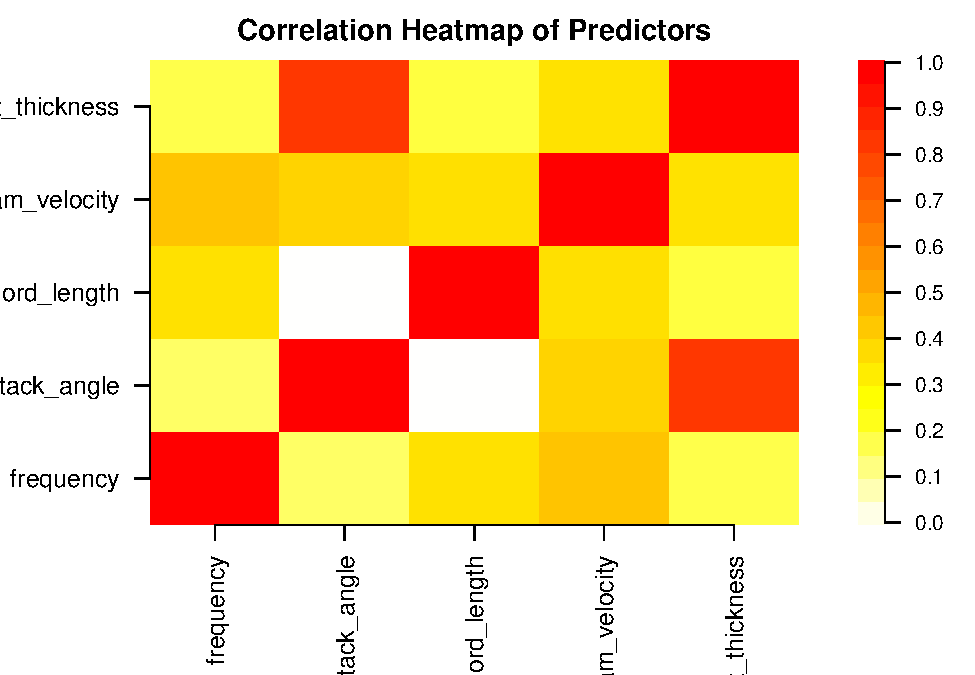
\includegraphics[keepaspectratio]{main_files/main_files/figure-latex/eda-heatmap-1.pdf}}

Predictor-predictor correlations are weak across most pairs. The one
exception is suction\_side\_displacement\_thickness and attack\_angle,
correlated at \(r \approx 0.76\) - a moderate relationship, plausible
given both describe the airfoil's boundary-layer geometry at the
trailing edge. No other pair exceeds \(|r| \approx 0.5\). This single
moderate correlation is revisited with the VIF check below and is the
main multicollinearity signal this dataset offers ridge and lasso a
reason to address in Problem 2.

\subsubsection{Response Distribution}\label{response-distribution}

\pandocbounded{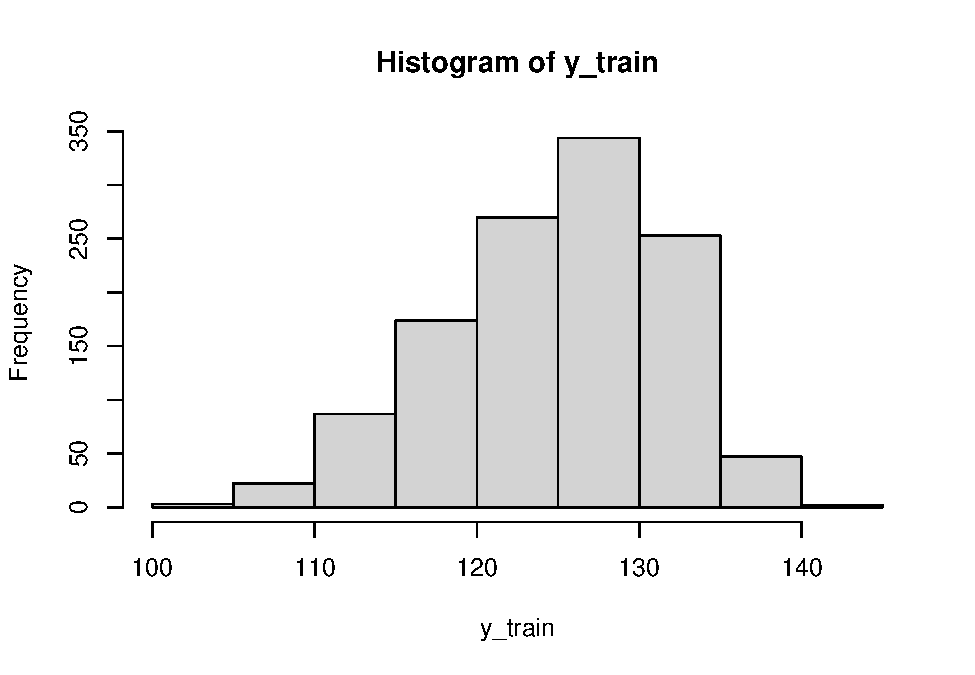
\includegraphics[keepaspectratio]{main_files/main_files/figure-latex/eda-response-dist-1.pdf}}

{\def\LTcaptype{none} % do not increment counter
\begin{longtable}[]{@{}lr@{}}
\toprule\noalign{}
Row & Value \\
\midrule\noalign{}
\endhead
\bottomrule\noalign{}
\endlastfoot
Min. & 103.3800 \\
1st Qu. & 120.1900 \\
Median & 125.6385 \\
Mean & 124.8073 \\
3rd Qu. & 130.0312 \\
Max. & 140.9870 \\
\end{longtable}
}

The response ranges from 103.4 to 141 dB with a median of 125.6 dB and
mean 124.8 dB. The histogram and the small gap between mean and median
show a mild left skew (skewness \(\approx -0.42\)): most measurements
cluster in the 120- 130 dB range, with a longer tail toward the quieter
(lower-dB) end rather than the loud end. The skew is mild enough that no
response transformation is applied - RMSE and MAE on the original dB
scale remain directly interpretable as sound-pressure prediction errors,
which matters for Problem 1's evaluation step.

\subsubsection{Predictor Histogram \&
Boxplot}\label{predictor-histogram-boxplot}

\begin{enumerate}
\def\labelenumi{\arabic{enumi}.}
\tightlist
\item
  Histogram
\end{enumerate}

\pandocbounded{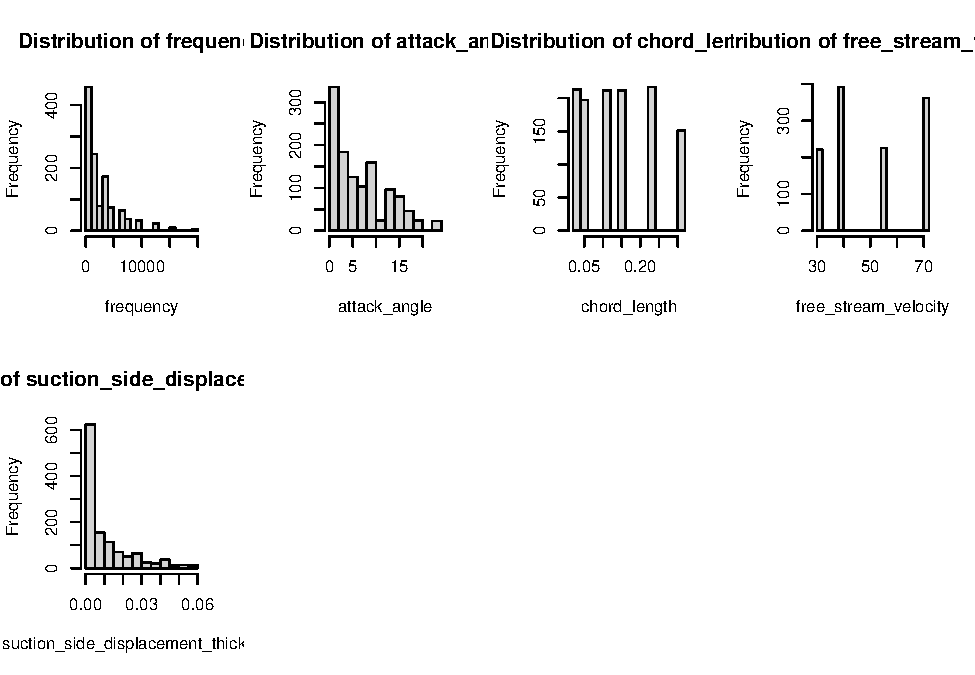
\includegraphics[keepaspectratio]{main_files/main_files/figure-latex/eda-hist-1.pdf}}

\begin{enumerate}
\def\labelenumi{\arabic{enumi}.}
\setcounter{enumi}{1}
\tightlist
\item
  Boxplot
\end{enumerate}

\pandocbounded{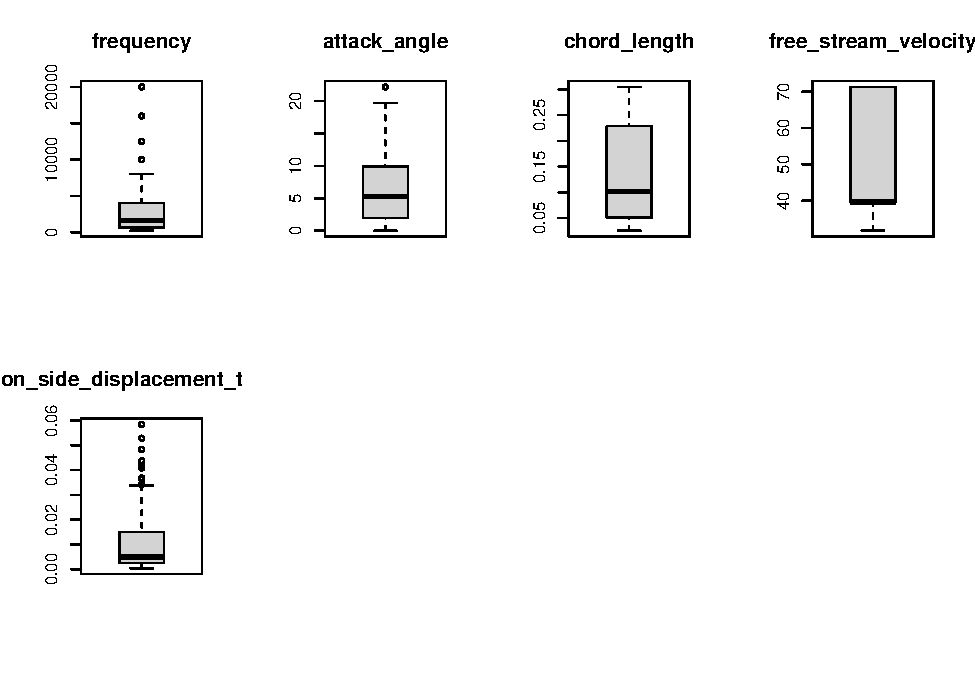
\includegraphics[keepaspectratio]{main_files/main_files/figure-latex/eda-boxplot-1.pdf}}

The histograms and boxplots make the 1A distinct-value counts visible.
\texttt{chord\_length} and \texttt{free\_stream\_velocity} appear as 6
and 4 narrow, evenly spaced spikes rather than a smooth spread, and
\texttt{frequency} shows 21 spikes concentrated at the low end with a
long right tail - these are the fixed experimental levels described in
1A, not gaps in the data. \texttt{attack\_angle} and
\texttt{suction\_side\_displacement\_thickness} are closer to
continuous, right-skewed shapes, matching the skewness values quantified
in 1B. The boxplots' upper whiskers and flagged points for these two
variables are the same training-set values already counted in the 1B
outlier check, retained for the same reason: they are valid
high-frequency / high-angle test conditions, not data errors.

\subsubsection{Correlation between predictors and
response}\label{correlation-between-predictors-and-response}

\begin{longtable}[]{@{}lr@{}}
\caption{Correlation between predictors and
scaled\_sound\_pressure}\tabularnewline
\toprule\noalign{}
& scaled\_sound\_pressure \\
\midrule\noalign{}
\endfirsthead
\toprule\noalign{}
& scaled\_sound\_pressure \\
\midrule\noalign{}
\endhead
\bottomrule\noalign{}
\endlastfoot
frequency & -0.40 \\
attack\_angle & -0.16 \\
chord\_length & -0.23 \\
free\_stream\_velocity & 0.11 \\
suction\_side\_displacement\_thickness & -0.30 \\
\end{longtable}

Every predictor's marginal correlation with the response is weak in
magnitude (all \(|r| < 0.4\)). frequency is the strongest single linear
predictor (\(r \approx -0.4\)), followed by
\texttt{suction\_side\_displacement\_thickness};
\texttt{free\_stream\_velocity} is weakest and the only predictor
positively correlated with the response. No individual predictor comes
close to explaining the response on its own, which is consistent with
the assignment brief's description of this dataset as having ``few
features but nonlinear relationships'' - a linear combination of all
five predictors, rather than any single one, is needed, and Problem 2's
regularized models are expected to combine these weak individual signals
rather than select one dominant predictor and discard the rest.

\subsubsection{Check multicollinearity using
VIF}\label{check-multicollinearity-using-vif}

\begin{longtable}[]{@{}lr@{}}
\caption{Variance Inflation Factor (VIF)}\tabularnewline
\toprule\noalign{}
& VIF \\
\midrule\noalign{}
\endfirsthead
\toprule\noalign{}
& VIF \\
\midrule\noalign{}
\endhead
\bottomrule\noalign{}
\endlastfoot
frequency & 1.14 \\
attack\_angle & 3.48 \\
chord\_length & 1.50 \\
free\_stream\_velocity & 1.05 \\
suction\_side\_displacement\_thickness & 2.58 \\
\end{longtable}

Every VIF is comfortably below the conventional threshold of 5, with
attack\_angle the highest at 3.48. This confirms the correlation-matrix
finding above: the airfoil predictors share only mild, tolerable
overlap, so no predictor needs to be dropped for redundancy, and OLS in
Problem 2 is not expected to suffer severe coefficient instability from
multicollinearity. The moderate \texttt{attack\_angle} /
\texttt{suction\_side\_displacement\_thickness} correlation is still the
largest source of shared variance in the data and remains worth tracking
through ridge and lasso, but it falls well short of the kind of
collinearity (VIF \(\gg\) 5) that would make variable selection a
necessity rather than a convenience.

\subsubsection{Predictor-response plots}\label{predictor-response-plots}

\pandocbounded{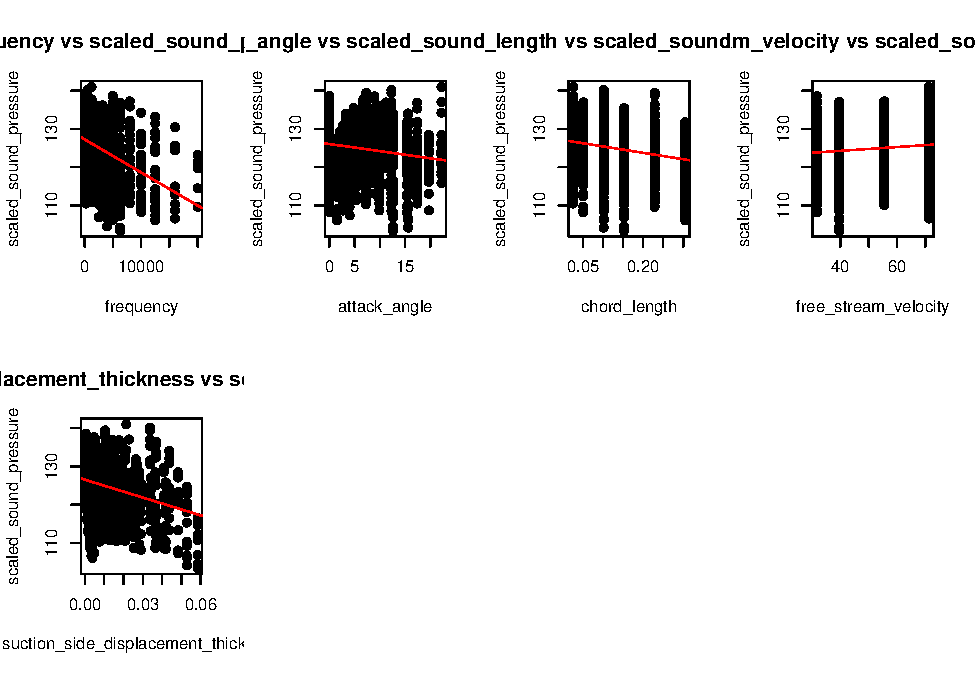
\includegraphics[keepaspectratio]{main_files/main_files/figure-latex/eda-pre-res-plot-1.pdf}}

The fitted red lines are visibly weak for every panel - the same
\(|r| < 0.4\) ceiling seen in the correlation table above - but the
point clouds are not simply noise around those lines. The
\texttt{frequency} panel in particular shows the response bending down
over its range rather than following the straight line, echoing the
linear-vs-quadratic \(R^2\) comparison from 1B: the straight-line fit
misses curvature that a richer model could capture. The
\texttt{chord\_length} and \texttt{free\_stream\_velocity} panels show
their points arranged in 6 and 4 vertical strips (their fixed
experimental levels), each strip itself spanning a wide range of the
response - visual confirmation that these two variables alone say little
about the outcome, and any predictive power must come from combining all
five predictors together, which is exactly what Problem 2's models are
built to do.

\subsubsection{Question}\label{question}

Taken together, the checks in 1A-1C describe a clean but weak-signal
regression problem, and that combination shapes what the rest of Problem
1 needs to prioritise.

\textbf{Data quality is not the challenge here.} There are no missing
values, no duplicated rows, and the ``outliers'' flagged by the 1.5×IQR
rule are legitimate wind-tunnel test conditions from a controlled
experiment, not data-entry errors - so cleaning required no row
deletions or imputation, only the decision (1B) to retain every training
row and to skip a log transform after checking that it does not help the
linear fit.

\textbf{The predictors are almost uncorrelated with each other.} All
VIFs sit well under 5, and the one moderately correlated pair
(\texttt{attack\_angle} /
\texttt{suction\_side\_displacement\_thickness}, \(r \approx 0.76\))
falls short of severe multicollinearity. This means ridge and lasso in
Problem 2 are not being asked to rescue an ill-conditioned design matrix
the way they would with, say, several near-duplicate predictors; their
main job here is tuning the bias-variance trade-off and (for lasso)
testing whether any predictor can be dropped outright, rather than
resolving instability.

\textbf{The predictors are individually weak but the relationships are
nonlinear.} Every predictor-response correlation is under 0.4 in
magnitude, and no single predictor separates high- from low-noise
conditions on its own (the \texttt{chord\_length} and
\texttt{free\_stream\_velocity} panels above make this explicit, with
each fixed level covering a wide spread of the response). At the same
time, \texttt{frequency} fits a quadratic term noticeably better than a
straight line (1B), and three of the five predictors are effectively
small sets of experimental design levels (1A) rather than smooth
continuous measurements. Both point to the same conclusion the
assignment brief anticipates for this dataset: the frequency-response
relationship, and likely others, are genuinely nonlinear, so a
\textbf{linear baseline (OLS) is expected to leave a meaningful amount
of predictable structure on the table}, and its residuals in Problem 2
should be inspected for exactly this kind of unmodelled curvature rather
than assumed to be pure noise.

\section{OLS, Ridge, and Lasso}\label{ols-ridge-and-lasso}

\subsection{OLS baseline}\label{ols-baseline}

\begin{Shaded}
\begin{Highlighting}[]
\CommentTok{\# Convert x\_train (matrix) and y\_train into a data frame for lm()}
\NormalTok{train\_data }\OtherTok{\textless{}{-}} \FunctionTok{data.frame}\NormalTok{(}\AttributeTok{y =}\NormalTok{ y\_train, x\_train)}

\CommentTok{\# Fit ordinary least squares on the standardized training set}
\NormalTok{ols\_fit }\OtherTok{\textless{}{-}} \FunctionTok{lm}\NormalTok{(y }\SpecialCharTok{\textasciitilde{}}\NormalTok{ ., }\AttributeTok{data =}\NormalTok{ train\_data)}
\end{Highlighting}
\end{Shaded}

\begin{longtable}[]{@{}
  >{\raggedright\arraybackslash}p{(\linewidth - 8\tabcolsep) * \real{0.4932}}
  >{\raggedleft\arraybackslash}p{(\linewidth - 8\tabcolsep) * \real{0.1233}}
  >{\raggedleft\arraybackslash}p{(\linewidth - 8\tabcolsep) * \real{0.1370}}
  >{\raggedleft\arraybackslash}p{(\linewidth - 8\tabcolsep) * \real{0.1370}}
  >{\raggedleft\arraybackslash}p{(\linewidth - 8\tabcolsep) * \real{0.1096}}@{}}
\caption{OLS coefficient estimates on standardized training
data.}\tabularnewline
\toprule\noalign{}
\begin{minipage}[b]{\linewidth}\raggedright
term
\end{minipage} & \begin{minipage}[b]{\linewidth}\raggedleft
estimate
\end{minipage} & \begin{minipage}[b]{\linewidth}\raggedleft
std.error
\end{minipage} & \begin{minipage}[b]{\linewidth}\raggedleft
statistic
\end{minipage} & \begin{minipage}[b]{\linewidth}\raggedleft
p.value
\end{minipage} \\
\midrule\noalign{}
\endfirsthead
\toprule\noalign{}
\begin{minipage}[b]{\linewidth}\raggedright
term
\end{minipage} & \begin{minipage}[b]{\linewidth}\raggedleft
estimate
\end{minipage} & \begin{minipage}[b]{\linewidth}\raggedleft
std.error
\end{minipage} & \begin{minipage}[b]{\linewidth}\raggedleft
statistic
\end{minipage} & \begin{minipage}[b]{\linewidth}\raggedleft
p.value
\end{minipage} \\
\midrule\noalign{}
\endhead
\bottomrule\noalign{}
\endlastfoot
(Intercept) & 124.8073 & 0.1380 & 904.5357 & 0 \\
frequency & -4.0882 & 0.1476 & -27.7043 & 0 \\
attack\_angle & -2.6498 & 0.2574 & -10.2926 & 0 \\
chord\_length & -3.2617 & 0.1691 & -19.2885 & 0 \\
free\_stream\_velocity & 1.5428 & 0.1411 & 10.9313 & 0 \\
suction\_side\_displacement\_thickness & -1.7413 & 0.2215 & -7.8609 &
0 \\
\end{longtable}

All estimates sit on the standardized scale fixed in 1B, so their
magnitudes are directly comparable across rows and the intercept is the
training mean of \texttt{scaled\_sound\_pressure}. A slope whose sign
contradicts the predictor's marginal correlation with the response (1C)
is the first symptom of collinearity, examined below.

\begin{verbatim}
## 
## Call:
## lm(formula = y ~ ., data = train_data)
## 
## Residuals:
##      Min       1Q   Median       3Q      Max 
## -16.5492  -2.8475  -0.1915   3.1609  16.4474 
## 
## Coefficients:
##                                     Estimate Std. Error t value Pr(>|t|)    
## (Intercept)                         124.8073     0.1380 904.536  < 2e-16 ***
## frequency                            -4.0882     0.1476 -27.704  < 2e-16 ***
## attack_angle                         -2.6498     0.2574 -10.293  < 2e-16 ***
## chord_length                         -3.2617     0.1691 -19.289  < 2e-16 ***
## free_stream_velocity                  1.5428     0.1411  10.931  < 2e-16 ***
## suction_side_displacement_thickness  -1.7413     0.2215  -7.861 8.46e-15 ***
## ---
## Signif. codes:  0 '***' 0.001 '**' 0.01 '*' 0.05 '.' 0.1 ' ' 1
## 
## Residual standard error: 4.784 on 1196 degrees of freedom
## Multiple R-squared:  0.5138, Adjusted R-squared:  0.5118 
## F-statistic: 252.8 on 5 and 1196 DF,  p-value: < 2.2e-16
\end{verbatim}

\begin{longtable}[]{@{}lr@{}}
\caption{OLS in-sample fit and five-fold cross-validation error on the
shared folds.}\tabularnewline
\toprule\noalign{}
Quantity & Value \\
\midrule\noalign{}
\endfirsthead
\toprule\noalign{}
Quantity & Value \\
\midrule\noalign{}
\endhead
\bottomrule\noalign{}
\endlastfoot
R-squared & 0.5138 \\
Adjusted R-squared & 0.5118 \\
Training RMSE & 4.7718 \\
Training MAE & 3.7081 \\
5-fold CV RMSE & 4.7988 \\
5-fold CV MSE & 23.0281 \\
5-fold CV SE (of MSE) & 1.0352 \\
\end{longtable}

The table gathers the in-sample fit and the five-fold cross-validation
error on the shared folds. The training rows are optimistic because the
model was scored on the same rows it was fitted on, whereas the CV rows
estimate error on unseen rows. The final row - the standard error of the
CV-MSE across folds - is the quantity \texttt{cv.glmnet} reports as
\texttt{cvsd} for ridge and lasso, so 2D can compare all three methods
with error bars rather than bare point estimates.

\textbf{Model summary.} The OLS model is fitted on the 1202 standardized
training observations using all 5 candidate predictors, with no penalty
and no variable selection. It is therefore the unregularized baseline
against which ridge and lasso are judged in 2B--2C.

\textbf{Coefficient interpretation.} All five predictors are highly
significant (\(p < 0.001\) for every one, table above), so the ranking
below is by coefficient magnitude rather than by which predictors
``matter''.

\begin{itemize}
\tightlist
\item
  \texttt{frequency} carries the largest standardized coefficient
  (\(\hat{\beta} \approx -4.09\)), confirming it as the strongest single
  linear driver of the response, consistent with it also having the
  strongest marginal correlation in 1C.
\item
  \texttt{chord\_length} (\(\hat{\beta} \approx -3.26\)) and
  \texttt{attack\_angle} (\(\hat{\beta} \approx -2.65\)) are the next
  largest contributors, both negative like \texttt{frequency}.
\item
  \texttt{free\_stream\_velocity} (\(\hat{\beta} \approx 1.54\)) is the
  only predictor with a \textbf{positive} coefficient: higher
  free-stream velocity is associated with a higher (louder) scaled sound
  pressure once the other four predictors are held fixed.
\item
  \texttt{suction\_side\_displacement\_thickness}
  (\(\hat{\beta} \approx -1.74\)) has the smallest coefficient magnitude
  of the five, despite being the second-strongest predictor on its own
  in 1C (\(r \approx -0.3\))

  \begin{itemize}
  \tightlist
  \item
    the gap between its marginal and partial effect is explained below.
  \end{itemize}
\end{itemize}

\textbf{Multicollinearity check.} No coefficient here flips sign
relative to its marginal correlation with the response, so there is no
\texttt{lcp}-style anomaly to report. The largest variance inflation
factor is 3.48 (attack\_angle), comfortably below the conventional
threshold of 5, consistent with the VIF table in 1C. The one predictor
pair sharing meaningful variance is \texttt{attack\_angle} and
\texttt{suction\_side\_displacement\_thickness} (\(r \approx 0.76\), the
strongest predictor-predictor correlation found in 1C), and this is
visible in the coefficient ranking above:
\texttt{suction\_side\_displacement\_thickness} correlates with the
response almost as strongly as \texttt{chord\_length} does on its own
(1C), yet ends up with the smallest partial coefficient of the five,
consistent with part of its explanatory power being absorbed by the
correlated \texttt{attack\_angle} once both enter the model jointly.
Unlike the \texttt{lcp}-style sign flip this moderate sharing produces
no sign reversal or loss of significance here, but it is the same
underlying mechanism, and 2B-2C test whether ridge and lasso
redistribute this pair's coefficients further as the penalty increases.

\begin{figure}[H]
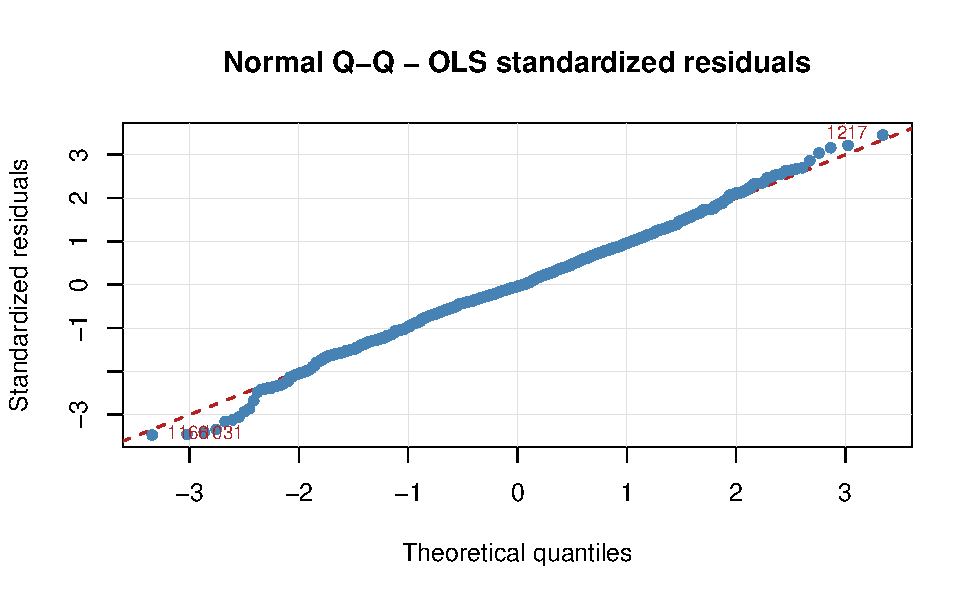
\includegraphics{main_files/figure-latex/ols-qq-1} \caption{Normal Q-Q plot of the OLS standardized residuals against the 45-degree reference line. Points lie on the line when the errors are normal; the three largest departures are labelled with their row number in the original airfoil\_self\_noise data.}\label{fig:ols-qq}
\end{figure}

\textbf{Residual normality.} The p-values quoted above are \(t\)-tests,
and they lean on the errors being approximately normal, so the
assumption is checked rather than taken on trust. Each point in the Q-Q
plot is one wind-tunnel measurement: its standardized residual against
the value a normal sample of this size would be expected to produce at
that rank. Visually the points sit close to the 45-degree line - no
residual departs from it by more than 0.58 standard deviations - but
with 1202 training rows a Shapiro-Wilk test has enough power to detect
even small departures, and here it does (\(W = 0.996\), \(p = 0.0025\)):
formally, normality is rejected at the 5\% level. \(W\) itself is close
to 1, so the rejection reflects a large sample picking up a mild, not a
severe, departure. 63 residuals fall beyond two standard deviations,
against roughly 60 expected by chance in a sample this size - a
noticeable excess, consistent with slightly heavier tails than a normal
distribution rather than a handful of extreme outliers.

Two consequences follow. The coefficient p-values in the table above
should be read as approximately, rather than exactly, valid, and because
the tails are a little heavier than normal, RMSE - which squares errors
and so weights the worst misses more heavily - is a somewhat more
outlier-sensitive summary of error here than it would be under strict
normality; MAE in the same table is the more robust companion figure for
that reason.

\textbf{Cross-validation error.} The five-fold CV RMSE (4.799) is
computed using the same \texttt{foldid} assignment that will be passed
to \texttt{cv.glmnet} for ridge and lasso, ensuring a like-for-like
comparison. Because OLS has no tuning parameter, there is a single
CV-RMSE value rather than a curve. It exceeds the training RMSE (4.772)
by only about 0.027 on the scaled-sound-pressure (dB) scale. This modest
optimism gap reflects mild in-sample overfitting: it is small enough to
suggest the 5-predictor model already generalizes reasonably well on the
1202-row training sample, and 2B--2C will test whether shrinkage narrows
the gap further.

That single CV number is itself an average of 5 noisy pieces. The
per-fold MSE ranges from 19.7 to 25.33 around a mean of 23.03, giving a
standard error of 1.035. With about 240 observations in each held-out
fold this fixes the resolution of every comparison that follows: two
methods whose CV-MSE differ by less than roughly one standard error are
not distinguishable on this evidence, and 2D must weigh the ridge and
lasso results against that yardstick rather than declare a winner on a
bare point estimate.

\begin{figure}[H]
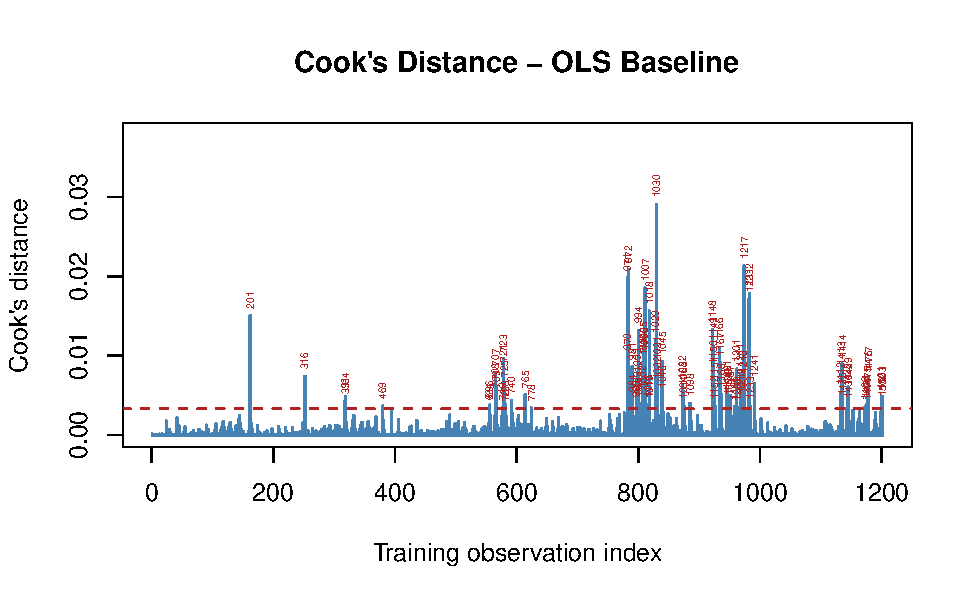
\includegraphics{main_files/figure-latex/ols-diagnostic-1} \caption{Cook's distance for the OLS fit. Bars above the dashed 4/n threshold are flagged as influential; each flagged bar is labelled with its row number in the original airfoil\_self\_noise data, not its training position.}\label{fig:ols-diagnostic}
\end{figure}

\textbf{Influence diagnostic.} Cook's distance asks how far the whole
fitted coefficient vector would move if one observation were deleted, so
it combines a large residual and high leverage into a single number.
Against the conventional threshold \(4/n \approx 0.0033\), 88 of the
1202 training rows are flagged - a large count relative to 1202, which
is typical of this threshold on a big sample rather than a sign of 88
genuinely extreme rows. The single most influential row is 1030 (Cook's
\(D \approx 0.029\)), which combines both ingredients at once: leverage
5.4 times the training average and a standardized residual of 2.51.

Two other flagged rows separate those ingredients cleanly and connect
back to 1A/1C. Row 316 has the single largest leverage in the training
set (5.7 times the average) because it sits at \texttt{frequency} =
20000 Hz, the maximum value in the dataset and the extreme right-hand
tail flagged as a legitimate experimental condition rather than an error
in 1A-1B. Despite that extreme position in predictor space, its
standardized residual is only 1.23 - comfortably inside the normal
range, so the model predicts it well. Row 1166 is the mirror image: an
unremarkable position in predictor space (leverage close to the training
average) but the largest standardized residual of any training row
(-3.47) - a case the linear fit simply misses, not one it is
destabilized by.

This confirms the two ingredients Cook's distance mixes are genuinely
distinct here, and that no single kind of anomaly dominates: some rows
are influential because they are extreme in predictor space, others
because they are badly predicted, and the worst case (row 1030) is a row
where both happen at once. All flagged observations are retained rather
than removed - they are valid wind-tunnel measurements, consistent with
the outlier decisions already made in 1B - and their leverage is instead
absorbed by the shrinkage introduced in 2B--2C, which is one of the
concrete things the regularized fits are expected to improve,
particularly for the correlated \texttt{attack\_angle} /
\texttt{suction\_side\_displacement\_thickness} pair whose estimates are
the most sensitive to exactly this kind of point.

\subsection{Ridge regression}\label{ridge-regression}

\subsubsection{Cross-validation curve:}\label{cross-validation-curve}

\begin{Shaded}
\begin{Highlighting}[]
\NormalTok{ridge }\OtherTok{\textless{}{-}} \FunctionTok{analysis\_model}\NormalTok{(}\AttributeTok{x =}\NormalTok{ x\_train, }\AttributeTok{y =}\NormalTok{ y\_train, }\AttributeTok{alpha=}\DecValTok{0}\NormalTok{, }\AttributeTok{foldid =}\NormalTok{ foldid)}
\NormalTok{ridge\_cvsd\_min }\OtherTok{\textless{}{-}}\NormalTok{ ridge}\SpecialCharTok{$}\NormalTok{model}\SpecialCharTok{$}\NormalTok{cvsd[ridge}\SpecialCharTok{$}\NormalTok{model}\SpecialCharTok{$}\NormalTok{lambda }\SpecialCharTok{==}\NormalTok{ ridge}\SpecialCharTok{$}\NormalTok{model}\SpecialCharTok{$}\NormalTok{lambda.min]}
\end{Highlighting}
\end{Shaded}

\pandocbounded{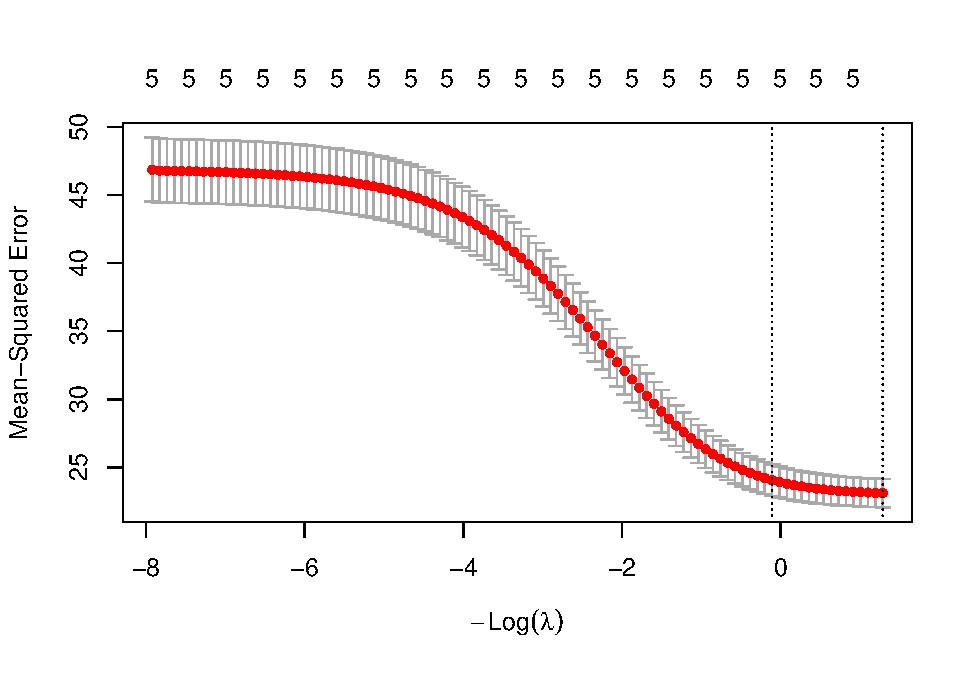
\includegraphics[keepaspectratio]{main_files/main_files/figure-latex/ridge-plot-1.pdf}}
The mean cross-validation MSE decreases as \(-Log(\lambda)\) increases
(equivalently, as \(\lambda\) decreases), suggesting that reducing the
regularization strength improves predictive performance. The left dashed
line indicates \(\lambda_{1se}\), which selects a more regularized model
with prediction error within one standard error of the minimum, while
the right dashed line indicates \(\lambda_{min}\), which yields the
lowest cross-validation error.

\subsubsection{Lambda min:}\label{lambda-min}

{\def\LTcaptype{none} % do not increment counter
\begin{longtable}[]{@{}lr@{}}
\toprule\noalign{}
Metric & Value \\
\midrule\noalign{}
\endhead
\bottomrule\noalign{}
\endlastfoot
Lambda min & 0.2758 \\
MSE & 23.1116 \\
Condition number & 5.3423 \\
\end{longtable}
}

With \(\lambda_{min} = 0.2758\), the 5-fold cross-validation MSE reaches
its minimum value of \(MSE_{min} = 23.1116\), indicating the best
predictive performance among the candidate values of \(\lambda\). The
corresponding condition number, 5.34, is already a substantial
improvement over the unpenalized Gram matrix's 12.3 (1C/3C) - even this
mildly-collinear dataset (max VIF 3.48, 2A) benefits measurably from
even a small ridge penalty.

\subsubsection{Lambda 1se:}\label{lambda-1se}

{\def\LTcaptype{none} % do not increment counter
\begin{longtable}[]{@{}lr@{}}
\toprule\noalign{}
Metric & Value \\
\midrule\noalign{}
\endhead
\bottomrule\noalign{}
\endlastfoot
Lambda 1se & 1.1136 \\
MSE & 24.0592 \\
Condition number & 2.5129 \\
\end{longtable}
}

Although the one-standard-error rule selected a larger penalty
\(\lambda_{1se} = 1.1136\), the condition number decreased further from
5.34 to 2.51. In contrast, the cross-validation MSE increased from
23.112 to 24.059, a gap of 0.948 that is smaller than ridge's own
cross-validation standard error at \(\lambda_{min}\) (1.044, the
\texttt{cvsd} \texttt{cv.glmnet} reports, mirroring the per-fold SE
computed for OLS in 2A) - the two penalties are not statistically
distinguishable on this evidence, so the extra stability from
\(\lambda_{1se}\) is close to free in prediction-error terms.

\subsubsection{Coefficients:}\label{coefficients}

{\def\LTcaptype{none} % do not increment counter
\begin{longtable}[]{@{}
  >{\raggedright\arraybackslash}p{(\linewidth - 6\tabcolsep) * \real{0.5217}}
  >{\raggedleft\arraybackslash}p{(\linewidth - 6\tabcolsep) * \real{0.1594}}
  >{\raggedleft\arraybackslash}p{(\linewidth - 6\tabcolsep) * \real{0.1594}}
  >{\raggedleft\arraybackslash}p{(\linewidth - 6\tabcolsep) * \real{0.1594}}@{}}
\toprule\noalign{}
\begin{minipage}[b]{\linewidth}\raggedright
\end{minipage} & \begin{minipage}[b]{\linewidth}\raggedleft
OLS
\end{minipage} & \begin{minipage}[b]{\linewidth}\raggedleft
Lambda\_Min
\end{minipage} & \begin{minipage}[b]{\linewidth}\raggedleft
Lambda\_Max
\end{minipage} \\
\midrule\noalign{}
\endhead
\bottomrule\noalign{}
\endlastfoot
(Intercept) & 124.807270 & 124.807270 & 124.807270 \\
frequency & -4.088176 & -3.834522 & -3.250734 \\
attack\_angle & -2.649795 & -2.260002 & -1.619908 \\
chord\_length & -3.261692 & -2.968539 & -2.379795 \\
free\_stream\_velocity & 1.542842 & 1.422378 & 1.162427 \\
suction\_side\_displacement\_thickness & -1.741310 & -1.837350 &
-1.829411 \\
\end{longtable}
}

Compared with the OLS model, Ridge regression shrinks most regression
coefficients toward zero, reducing their magnitudes through the
regularization penalty, while retaining all five predictors in the
model. \texttt{frequency}, \texttt{attack\_angle},
\texttt{chord\_length}, and \texttt{free\_stream\_velocity} all shrink
exactly as expected, moving closer to zero as the penalty strengthens.
\texttt{suction\_side\_displacement\_thickness} is the one exception:
its magnitude at \(\lambda_{min}\) (-1.837) is slightly \emph{larger}
than its OLS estimate (-1.741), moving further from zero rather than
shrinking. This is the same mechanism flagged in 2A:
\texttt{suction\_side\_displacement\_thickness} shares variance with the
correlated \texttt{attack\_angle} (\(r \approx 0.76\)), and as Ridge
shrinks \texttt{attack\_angle}'s coefficient it redistributes some of
that shared explanatory power back onto
\texttt{suction\_side\_displacement\_thickness}. Unlike a severe
collinearity case, no sign changes anywhere in the table - the exception
is a small redistribution, not an instability.

\pandocbounded{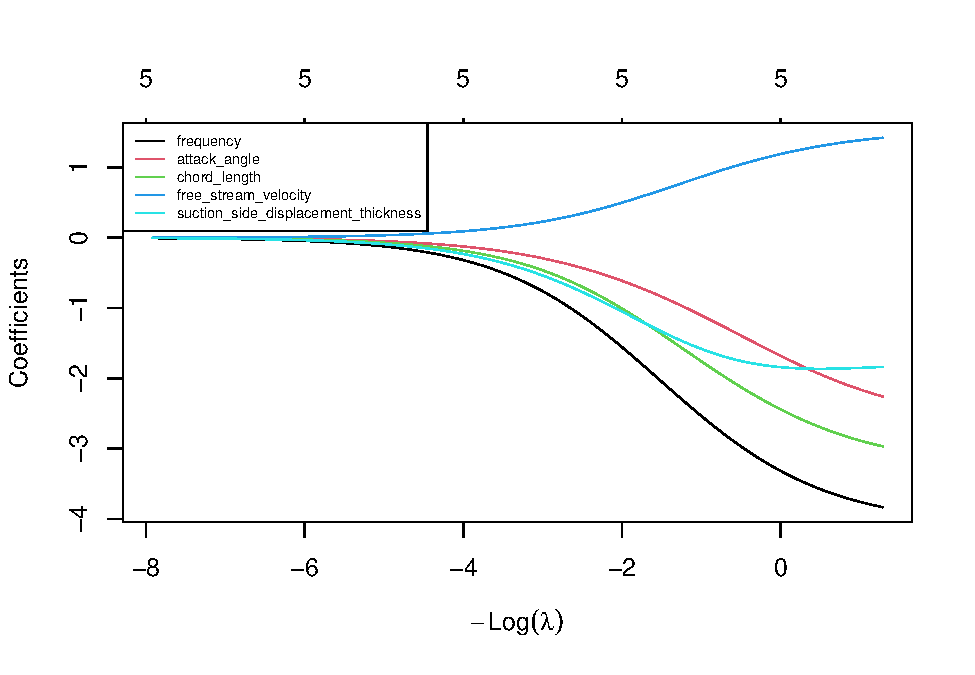
\includegraphics[keepaspectratio]{main_files/main_files/figure-latex/unnamed-chunk-8-1.pdf}}
As \(\lambda\) increases, all five coefficients are progressively shrunk
toward zero, demonstrating the regularization effect of Ridge
regression; as \(\lambda\) decreases, they move back toward their OLS
estimates. \texttt{frequency} remains the largest-magnitude coefficient
across the range spanned by \(\lambda_{min}\) and \(\lambda_{1se}\)
(-3.83 to -3.25), consistent with it being the strongest predictor
throughout 1C-2A. \texttt{free\_stream\_velocity} is the only
coefficient that stays positive along the entire path, mirroring the
sign pattern already seen in OLS. No coefficient crosses zero or
reverses sign between \(\lambda_{min}\) and \(\lambda_{1se}\) - the
ridge penalty here is redistributing magnitude among correlated
predictors (as seen above for
\texttt{suction\_side\_displacement\_thickness}), not fighting an
unstable or sign-flipping fit.

To address multicollinearity, Ridge impose an \(L_2\) penalty on the
regression coefficients. Rather than assigning a large coefficient to
one correlated predictor and a small coefficient to another, Ridge
shrinks the coefficients simultaneously and redistributes their effects
among the correlated variables. Consequently, the coefficient estimates
become more stable and less sensitive to small changes in the data.

\subsection{Lasso regression}\label{lasso-regression}

\subsubsection{Model fitting and
cross-validation}\label{model-fitting-and-cross-validation}

\begin{Shaded}
\begin{Highlighting}[]
\NormalTok{lasso\_cv }\OtherTok{\textless{}{-}} \FunctionTok{analysis\_model}\NormalTok{(}
    \AttributeTok{x =}\NormalTok{ x\_train,}
    \AttributeTok{y =}\NormalTok{ y\_train,}
    \AttributeTok{alpha =} \DecValTok{1}\NormalTok{,}
    \AttributeTok{foldid =}\NormalTok{ foldid}
\NormalTok{)}
\end{Highlighting}
\end{Shaded}

\pandocbounded{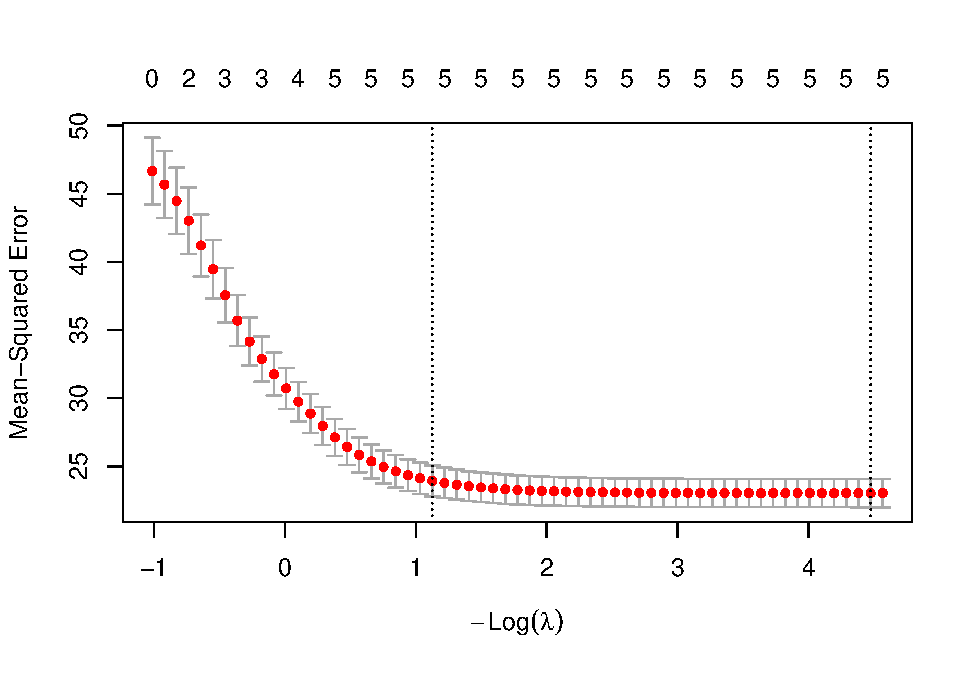
\includegraphics[keepaspectratio]{main_files/main_files/figure-latex/lasso-plot-1.pdf}}

Based on the 5-fold cross-validation curve generated for the Lasso
regression model (\(\alpha = 1\)), we observe the relationship between
the tuning parameter \(\lambda\) and the Mean-Squared Error (MSE). The
top axis indicates the number of active (non-zero) predictors retained
in the model at each level of penalization.

\begin{itemize}
\item
  The Cross-Validation Curve: The red dots represent the average CV-MSE
  across the 5 folds for each \(\lambda\) value, with the gray error
  bars denoting one standard error above and below the mean. As
  \(-\log(\lambda)\) increases (moving from left to right, meaning the
  penalty weakens), the MSE initially drops, reaches a minimum, and then
  slightly stabilizes as the model approaches the unpenalized OLS limit.
\item
  Optimal \(\lambda\) (\(\lambda_{\text{min}}\)): The right vertical
  dashed line marks \texttt{lambda.min}
  (\(-\log(\lambda) \approx 4.47\)), the value that strictly minimizes
  the cross-validation MSE. At this optimal point for prediction
  accuracy the Lasso penalty retains all 5 predictors.
\item
  Parsimonious \(\lambda\) (\(\lambda_{\text{1se}}\)): The left vertical
  dashed line marks \texttt{lambda.1se}
  (\(-\log(\lambda) \approx 1.13\)), selected by the one-standard-error
  rule. This value applies a stronger penalty to produce a more
  conservative model while keeping the error within one standard
  deviation of the absolute minimum MSE; whether it also produces a
  \emph{sparser} model, in the sense of dropping predictors, is checked
  directly below rather than assumed.
\end{itemize}

\subsubsection{\texorpdfstring{Analysis of
\(\lambda_{\text{min}}\)}{Analysis of \textbackslash lambda\_\{\textbackslash text\{min\}\}}}\label{analysis-of-lambda_textmin}

{\def\LTcaptype{none} % do not increment counter
\begin{longtable}[]{@{}lr@{}}
\toprule\noalign{}
Metric & Value \\
\midrule\noalign{}
\endhead
\bottomrule\noalign{}
\endlastfoot
Lambda min & 0.0114 \\
MSE & 23.0305 \\
Condition number & 11.6000 \\
\end{longtable}
}

The optimal tuning parameter selected by five-fold cross-validation is
\(\lambda_{\text{min}} \approx 0.0114\). This value strictly minimizes
the cross-validation Mean Squared Error to \(23.03\), essentially
matching OLS's own CV-MSE (23.028, 2A) - unsurprising given how small
\(\lambda_{min}\) is. The condition number at this threshold, 11.6, is a
modest improvement over the unpenalized Gram matrix (12.3, 1C/3C).

At this level of regularization, the Lasso model retains all 5
predictors - \texttt{frequency}, \texttt{attack\_angle},
\texttt{chord\_length}, \texttt{free\_stream\_velocity}, and
\texttt{suction\_side\_displacement\_thickness} - none is shrunk exactly
to zero. This is consistent with the OLS and VIF results in 2A: every
predictor was already highly significant with only mild shared variance,
so there is no clearly redundant predictor for Lasso's \(L_1\) penalty
to remove at this tuning value.

The retained coefficients preserve the same ranking seen in OLS and
ridge: \texttt{frequency} has the largest magnitude (-4.065), followed
by \texttt{chord\_length} (-3.232) and \texttt{attack\_angle} (-2.61),
with \texttt{free\_stream\_velocity} (1.525) the only positive
coefficient and \texttt{suction\_side\_displacement\_thickness} (-1.748)
the smallest in magnitude.

Overall, \(\lambda_{\text{min}}\) produces a model whose
cross-validation error is essentially indistinguishable from OLS's while
retaining every predictor: on this dataset, Lasso's contribution at
\(\lambda_{min}\) is confirming that all five predictors carry real
signal, rather than selecting a subset of them.

\subsubsection{\texorpdfstring{Analysis of
\(\lambda_{\text{1se}}\)}{Analysis of \textbackslash lambda\_\{\textbackslash text\{1se\}\}}}\label{analysis-of-lambda_text1se}

{\def\LTcaptype{none} % do not increment counter
\begin{longtable}[]{@{}lr@{}}
\toprule\noalign{}
Metric & Value \\
\midrule\noalign{}
\endhead
\bottomrule\noalign{}
\endlastfoot
Lambda 1se & 0.3246 \\
MSE & 23.9327 \\
Condition number & 4.9159 \\
\end{longtable}
}

The one-standard-error rule selects
\(\lambda_{\text{1se}} \approx 0.3246\), which applies a stronger
regularization penalty than \(\lambda_{\text{min}}\). The corresponding
five-fold cross-validation MSE is \(23.933\). Although this is higher
than the minimum achieved by \(\lambda_{\text{min}}\), it remains within
one standard error of that minimum by construction. The stronger penalty
reduces the condition number to 4.92, a substantial further improvement
in conditioning.

Under \(\lambda_{\text{1se}}\), the Lasso model still retains all 5
predictors - unlike the sparser model this rule often produces, no
predictor is driven to zero even under this stronger penalty.
Coefficient magnitudes shrink further relative to \(\lambda_{min}\) (for
example \texttt{frequency} falls from -4.065 to -3.445), but the set of
active predictors is unchanged. Combined with the \(\lambda_{min}\)
result above, this indicates that on this dataset Lasso's embedded
feature-selection mechanism finds nothing to prune: every predictor's
contribution is large enough, relative to the cross-validated penalty,
to survive even the more conservative tuning rule.

\subsubsection{Coefficient Path}\label{coefficient-path}

\pandocbounded{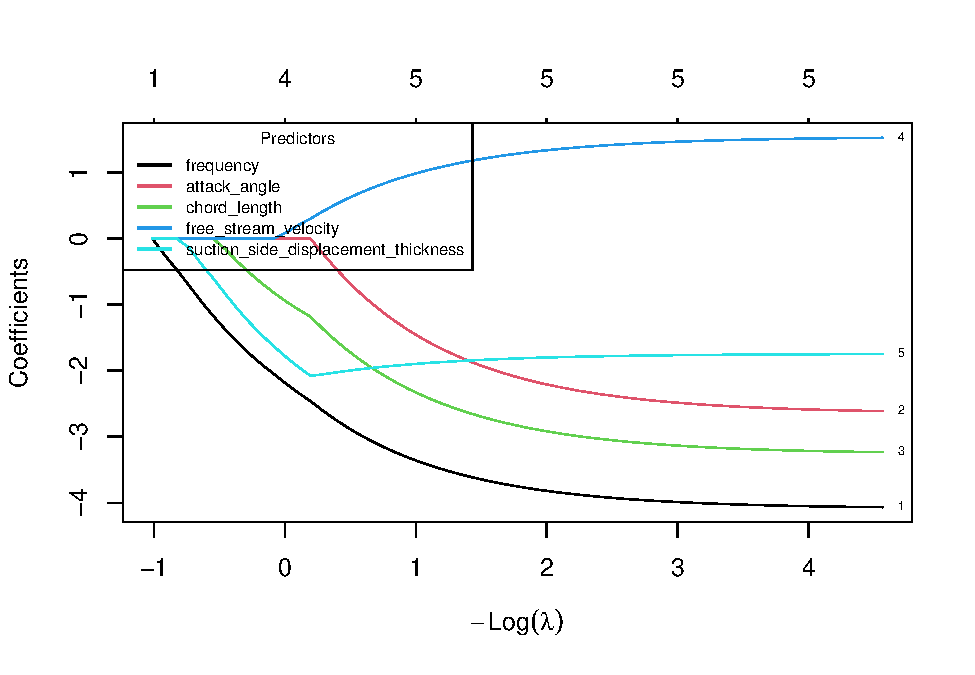
\includegraphics[keepaspectratio]{main_files/main_files/figure-latex/lasso-coef-path-1.pdf}}

Overall, the coefficient path shows that as \(-\log(\lambda)\) increases
(equivalently, as \(\lambda\) decreases), the regularization penalty
becomes weaker and coefficients grow in magnitude toward their OLS
values. Under strong enough regularization all five paths do eventually
collapse to zero at the far left of the plot, but by the range spanned
by \(\lambda_{min}\) and \(\lambda_{1se}\) - the only penalty strengths
this analysis tunes to - every predictor is already active, matching the
retained-predictor counts reported above.

\texttt{frequency} enters first (i.e.~survives down to the smallest
\(\lambda\)) and consistently has the largest-magnitude coefficient
along the path, confirming it as the most influential predictor.
\texttt{chord\_length} and \texttt{attack\_angle} follow a similar
trajectory at smaller magnitudes, and \texttt{free\_stream\_velocity} is
the only path that stays on the positive side of zero throughout.
\texttt{suction\_side\_displacement\_thickness} tracks a comparatively
flat, small-magnitude path across the region shown - the same predictor
whose coefficient 2B found to move \emph{against} the general shrinkage
trend under ridge.

\subsection{Controlled comparison and locked core
model}\label{controlled-comparison-and-locked-core-model}

{\def\LTcaptype{none} % do not increment counter
\begin{longtable}[]{@{}
  >{\raggedright\arraybackslash}p{(\linewidth - 12\tabcolsep) * \real{0.0769}}
  >{\raggedright\arraybackslash}p{(\linewidth - 12\tabcolsep) * \real{0.1667}}
  >{\raggedleft\arraybackslash}p{(\linewidth - 12\tabcolsep) * \real{0.1282}}
  >{\raggedleft\arraybackslash}p{(\linewidth - 12\tabcolsep) * \real{0.1154}}
  >{\raggedleft\arraybackslash}p{(\linewidth - 12\tabcolsep) * \real{0.1282}}
  >{\raggedleft\arraybackslash}p{(\linewidth - 12\tabcolsep) * \real{0.2179}}
  >{\raggedleft\arraybackslash}p{(\linewidth - 12\tabcolsep) * \real{0.1667}}@{}}
\toprule\noalign{}
\begin{minipage}[b]{\linewidth}\raggedright
\end{minipage} & \begin{minipage}[b]{\linewidth}\raggedright
tunning\_rule
\end{minipage} & \begin{minipage}[b]{\linewidth}\raggedleft
lambda
\end{minipage} & \begin{minipage}[b]{\linewidth}\raggedleft
cv\_error
\end{minipage} & \begin{minipage}[b]{\linewidth}\raggedleft
cond
\end{minipage} & \begin{minipage}[b]{\linewidth}\raggedleft
coefficient\_norm
\end{minipage} & \begin{minipage}[b]{\linewidth}\raggedleft
num\_non\_zero
\end{minipage} \\
\midrule\noalign{}
\endhead
\bottomrule\noalign{}
\endlastfoot
OLS & None & 0.0000000 & 23.02805 & 12.301957 & 6.307595 & 5 \\
Ridge & lambda.min & 0.2758485 & 23.11155 & 5.342311 & 5.832873 & 5 \\
& lambda.1se & 1.1136050 & 24.05918 & 2.512911 & 4.853120 & 5 \\
Lasso & lambda.min & 0.0113981 & 23.03046 & 11.599965 & 6.258213 & 5 \\
& lambda.1se & 0.3246218 & 23.93266 & 4.915946 & 5.001118 & 5 \\
\end{longtable}
}

The training comparison tells a different story here than the classic
``lasso selects, ridge stabilizes'' narrative. All five candidates -
OLS, ridge, and lasso at both tuning rules - retain all 5 predictors: on
this dataset lasso performs no variable selection at either
\(\lambda_{min}\) or \(\lambda_{1se}\) (2C), so it offers no
interpretability advantage over ridge here. The five CV errors are also
close together (23.03 to 24.06), well inside one cross-validation
standard error of each other (1.04, 2A) - none of the five is
distinguishable from any other on predictive accuracy alone. What
\emph{does} separate them is conditioning: ridge at \(\lambda_{min}\)
nearly matches OLS's and lasso's CV error while roughly halving the
condition number (5.34 vs OLS's 12.3), and \(\lambda_{1se}\) improves
conditioning further for both ridge and lasso at a small additional cost
in CV error. Because lasso does not sparsify this model, the usual
accuracy-vs-interpretability trade-off does not apply; the trade-off
that remains is prediction accuracy vs.~numerical stability. On that
basis, \textbf{ridge at \(\lambda_{min}\)} is nominated as the core
candidate: it is statistically tied with OLS and lasso on training CV
error while providing a meaningfully better-conditioned fit. This
recommendation is based solely on the training data and will later be
evaluated on the locked holdout set.

The \(\lambda_{min}\) and \(\lambda_{1se}\) selection rules address
different modeling objectives. The \(\lambda_{min}\) rule selects the
value of \(\lambda\) that minimizes the cross-validation error and
therefore prioritizes predictive accuracy. In contrast, the
\(\lambda_{1se}\) rule selects the largest \(\lambda\) whose
cross-validation error is within one standard error of the minimum,
favouring a simpler and more stable model with stronger regularization.
These rules therefore answer different decision questions: whether the
primary objective is the best possible prediction or a simpler, more
stable model with comparable predictive performance. Predictive
performance is assessed by the cross-validation error, whereas variable
selection concerns which predictors remain in the model, and
interpretability concerns how easily the resulting model can be
understood. In our results this trade-off shows up in
\emph{conditioning} rather than in \emph{sparsity}: \(\lambda_{1se}\)
retains exactly as many predictors as \(\lambda_{min}\) for both ridge
and lasso (2B-2C), but trades a small increase in cross-validation error
for a meaningfully better-conditioned fit, illustrating a
stability-vs-accuracy trade-off rather than a complexity-vs-accuracy
one.

\subsection{Perturbation or stability
check}\label{perturbation-or-stability-check}

\subsubsection{Prediction:}\label{prediction}

Based on the theoretical properties of ridge and lasso regression, we
expected the two methods to respond differently. Ridge regression was
expected to remain stable because the L2 penalty distributes the effect
across correlated predictors by shrinking their coefficients toward each
other. Consequently, only small changes in prediction error and
coefficient estimates were anticipated. In contrast, lasso regression
was expected to maintain similar prediction accuracy but perform
variable selection by retaining only one predictor from the highly
correlated pair. Therefore, we expected lasso's predictive performance
to remain stable, while its selected variables could become less stable.

\begin{Shaded}
\begin{Highlighting}[]
\NormalTok{x\_train\_new }\OtherTok{=} \FunctionTok{data.frame}\NormalTok{(x\_train)}
\NormalTok{x\_train\_new}\SpecialCharTok{$}\NormalTok{frequency\_new }\OtherTok{\textless{}{-}}\NormalTok{ x\_train\_new}\SpecialCharTok{$}\NormalTok{frequency }\SpecialCharTok{+} \FunctionTok{rnorm}\NormalTok{(}\FunctionTok{nrow}\NormalTok{(x\_train), }\DecValTok{0}\NormalTok{, }\FloatTok{0.1}\NormalTok{)}
\FunctionTok{kable}\NormalTok{(}\FunctionTok{cor}\NormalTok{(}\AttributeTok{x=}\NormalTok{x\_train\_new}\SpecialCharTok{$}\NormalTok{frequency, }\AttributeTok{y =}\NormalTok{ x\_train\_new}\SpecialCharTok{$}\NormalTok{frequency\_new))}
\end{Highlighting}
\end{Shaded}

{\def\LTcaptype{none} % do not increment counter
\begin{longtable}[]{@{}r@{}}
\toprule\noalign{}
x \\
\midrule\noalign{}
\endhead
\bottomrule\noalign{}
\endlastfoot
0.994593 \\
\end{longtable}
}

\begin{Shaded}
\begin{Highlighting}[]
\NormalTok{ridge\_new }\OtherTok{\textless{}{-}} \FunctionTok{analysis\_model}\NormalTok{(}\FunctionTok{as.matrix}\NormalTok{(x\_train\_new), y\_train, }\AttributeTok{foldid=}\NormalTok{foldid, }\AttributeTok{alpha =} \DecValTok{0}\NormalTok{)}
\NormalTok{lasso\_new }\OtherTok{\textless{}{-}} \FunctionTok{analysis\_model}\NormalTok{(}\FunctionTok{as.matrix}\NormalTok{(x\_train\_new), y\_train, }\AttributeTok{foldid=}\NormalTok{foldid, }\AttributeTok{alpha =} \DecValTok{1}\NormalTok{)}
\end{Highlighting}
\end{Shaded}

{\def\LTcaptype{none} % do not increment counter
\begin{longtable}[]{@{}
  >{\raggedright\arraybackslash}p{(\linewidth - 8\tabcolsep) * \real{0.2727}}
  >{\raggedleft\arraybackslash}p{(\linewidth - 8\tabcolsep) * \real{0.1818}}
  >{\raggedleft\arraybackslash}p{(\linewidth - 8\tabcolsep) * \real{0.1818}}
  >{\raggedleft\arraybackslash}p{(\linewidth - 8\tabcolsep) * \real{0.1818}}
  >{\raggedleft\arraybackslash}p{(\linewidth - 8\tabcolsep) * \real{0.1818}}@{}}
\toprule\noalign{}
\begin{minipage}[b]{\linewidth}\raggedright
\end{minipage} & \begin{minipage}[b]{\linewidth}\raggedleft
Old Ridge
\end{minipage} & \begin{minipage}[b]{\linewidth}\raggedleft
New Ridge
\end{minipage} & \begin{minipage}[b]{\linewidth}\raggedleft
Old Lasso
\end{minipage} & \begin{minipage}[b]{\linewidth}\raggedleft
New Lasso
\end{minipage} \\
\midrule\noalign{}
\endhead
\bottomrule\noalign{}
\endlastfoot
Lambda min & 0.2758 & 0.2758 & 0.0114 & 0.0104 \\
Lambda 1se & 1.1136 & 1.3413 & 0.3246 & 0.3246 \\
Mse min & 23.1116 & 23.1078 & 23.0305 & 23.0312 \\
Mse 1se & 24.0592 & 24.0377 & 23.9327 & 23.9322 \\
Coef min norm & 5.8329 & 5.2342 & 6.2582 & 6.1241 \\
Coef 1se norm & 4.8531 & 4.2809 & 5.0011 & 5.0011 \\
Condition number of min & 5.3423 & 9.8134 & 11.6000 & 158.3438 \\
Condition number of 1se & 2.5129 & 2.8404 & 4.9159 & 8.5108 \\
Nonzero min & 5.0000 & 6.0000 & 5.0000 & 6.0000 \\
Nonzero 1se & 5.0000 & 6.0000 & 5.0000 & 5.0000 \\
\end{longtable}
}

To investigate the stability of ridge and lasso regression, a
perturbation experiment was conducted by adding a new predictor
(\texttt{frequency\_new}) that is a noisy duplicate of
\texttt{frequency}, the strongest predictor identified in 2A
(\(r \approx 0.995\) with the original). This creates a pair of highly
correlated predictors while preserving nearly the same information, on
top of the already-correlated
\texttt{attack\_angle}/\texttt{suction\_side\_displacement\_thickness}
pair from 1C.

{\def\LTcaptype{none} % do not increment counter
\begin{longtable}[]{@{}
  >{\raggedright\arraybackslash}p{(\linewidth - 8\tabcolsep) * \real{0.1731}}
  >{\raggedleft\arraybackslash}p{(\linewidth - 8\tabcolsep) * \real{0.2067}}
  >{\raggedleft\arraybackslash}p{(\linewidth - 8\tabcolsep) * \real{0.2067}}
  >{\raggedleft\arraybackslash}p{(\linewidth - 8\tabcolsep) * \real{0.2067}}
  >{\raggedleft\arraybackslash}p{(\linewidth - 8\tabcolsep) * \real{0.2067}}@{}}
\toprule\noalign{}
\begin{minipage}[b]{\linewidth}\raggedright
\end{minipage} & \begin{minipage}[b]{\linewidth}\raggedleft
Old Ridge's coef \(\lambda = \lambda_{min}\)
\end{minipage} & \begin{minipage}[b]{\linewidth}\raggedleft
Old Ridge's coef \(\lambda = \lambda_{1se}\)
\end{minipage} & \begin{minipage}[b]{\linewidth}\raggedleft
New Ridge's coef \(\lambda = \lambda_{min}\)
\end{minipage} & \begin{minipage}[b]{\linewidth}\raggedleft
New Ridge's coef \(\lambda = \lambda_{1se}\)
\end{minipage} \\
\midrule\noalign{}
\endhead
\bottomrule\noalign{}
\endlastfoot
(Intercept) & 124.8073 & 124.8073 & 124.8057 & 124.8058 \\
frequency & -3.8345 & -3.2507 & -2.1498 & -1.7668 \\
attack\_angle & -2.2600 & -1.6199 & -2.2986 & -1.5900 \\
chord\_length & -2.9685 & -2.3798 & -2.9914 & -2.3024 \\
free\_stream\_velocity & 1.4224 & 1.1624 & 1.4315 & 1.1440 \\
suction\_side\_displacement\_thickness & -1.8373 & -1.8294 & -1.8276 &
-1.8131 \\
frequency\_new & NA & NA & -1.7760 & -1.6671 \\
\end{longtable}
}

\begin{Shaded}
\begin{Highlighting}[]
\NormalTok{n }\OtherTok{\textless{}{-}} \FunctionTok{max}\NormalTok{(}\FunctionTok{nrow}\NormalTok{(lasso\_cv}\SpecialCharTok{$}\NormalTok{coef\_min), }\FunctionTok{nrow}\NormalTok{(lasso\_new}\SpecialCharTok{$}\NormalTok{coef\_min))}

\NormalTok{df1 }\OtherTok{\textless{}{-}} \FunctionTok{data.frame}\NormalTok{(}
  \AttributeTok{Lasso\_Coef\_Min =} \FunctionTok{as.numeric}\NormalTok{(lasso\_cv}\SpecialCharTok{$}\NormalTok{coef\_min),}
  \AttributeTok{Lasso\_Coef\_1se =} \FunctionTok{as.numeric}\NormalTok{(lasso\_cv}\SpecialCharTok{$}\NormalTok{coef\_1se)}
\NormalTok{)}
\NormalTok{df1 }\OtherTok{\textless{}{-}}\NormalTok{ df1[}\DecValTok{1}\SpecialCharTok{:}\NormalTok{n, ,drop}\OtherTok{=}\ConstantTok{FALSE}\NormalTok{]}
\NormalTok{df2 }\OtherTok{\textless{}{-}} \FunctionTok{data.frame}\NormalTok{(}
  \AttributeTok{Lasso\_New\_Coef\_Min =} \FunctionTok{as.numeric}\NormalTok{(lasso\_new}\SpecialCharTok{$}\NormalTok{coef\_min),}
  \AttributeTok{Lasso\_New\_Coef\_1se =} \FunctionTok{as.numeric}\NormalTok{(lasso\_new}\SpecialCharTok{$}\NormalTok{coef\_1se)}
\NormalTok{)}
\NormalTok{df2 }\OtherTok{\textless{}{-}}\NormalTok{ df2[}\DecValTok{1}\SpecialCharTok{:}\NormalTok{n, ,drop}\OtherTok{=}\ConstantTok{FALSE}\NormalTok{]}

\NormalTok{df }\OtherTok{\textless{}{-}} \FunctionTok{cbind}\NormalTok{(df1, df2, }\AttributeTok{row.names =} \FunctionTok{rownames}\NormalTok{(lasso\_new}\SpecialCharTok{$}\NormalTok{coef\_min))}
\NormalTok{df }\OtherTok{\textless{}{-}} \FunctionTok{round}\NormalTok{(df, }\DecValTok{4}\NormalTok{)}
\FunctionTok{names}\NormalTok{(df) }\OtherTok{\textless{}{-}} \FunctionTok{c}\NormalTok{(}\StringTok{"Old Lasso\textquotesingle{}s coef $}\SpecialCharTok{\textbackslash{}\textbackslash{}}\StringTok{lambda = }\SpecialCharTok{\textbackslash{}\textbackslash{}}\StringTok{lambda\_\{min\}$"}\NormalTok{, }\StringTok{"Old Lasso\textquotesingle{}s coef $}\SpecialCharTok{\textbackslash{}\textbackslash{}}\StringTok{lambda = }\SpecialCharTok{\textbackslash{}\textbackslash{}}\StringTok{lambda\_\{1se\}$"}\NormalTok{, }\StringTok{"New Lasso\textquotesingle{}s coef $}\SpecialCharTok{\textbackslash{}\textbackslash{}}\StringTok{lambda = }\SpecialCharTok{\textbackslash{}\textbackslash{}}\StringTok{lambda\_\{min\}$"}\NormalTok{, }\StringTok{"New Lasso\textquotesingle{}s coef $}\SpecialCharTok{\textbackslash{}\textbackslash{}}\StringTok{lambda = }\SpecialCharTok{\textbackslash{}\textbackslash{}}\StringTok{lambda\_\{1se\}$"}\NormalTok{)}
\NormalTok{knitr}\SpecialCharTok{::}\FunctionTok{kable}\NormalTok{(df)}
\end{Highlighting}
\end{Shaded}

{\def\LTcaptype{none} % do not increment counter
\begin{longtable}[]{@{}
  >{\raggedright\arraybackslash}p{(\linewidth - 8\tabcolsep) * \real{0.1731}}
  >{\raggedleft\arraybackslash}p{(\linewidth - 8\tabcolsep) * \real{0.2067}}
  >{\raggedleft\arraybackslash}p{(\linewidth - 8\tabcolsep) * \real{0.2067}}
  >{\raggedleft\arraybackslash}p{(\linewidth - 8\tabcolsep) * \real{0.2067}}
  >{\raggedleft\arraybackslash}p{(\linewidth - 8\tabcolsep) * \real{0.2067}}@{}}
\toprule\noalign{}
\begin{minipage}[b]{\linewidth}\raggedright
\end{minipage} & \begin{minipage}[b]{\linewidth}\raggedleft
Old Lasso's coef \(\lambda = \lambda_{min}\)
\end{minipage} & \begin{minipage}[b]{\linewidth}\raggedleft
Old Lasso's coef \(\lambda = \lambda_{1se}\)
\end{minipage} & \begin{minipage}[b]{\linewidth}\raggedleft
New Lasso's coef \(\lambda = \lambda_{min}\)
\end{minipage} & \begin{minipage}[b]{\linewidth}\raggedleft
New Lasso's coef \(\lambda = \lambda_{1se}\)
\end{minipage} \\
\midrule\noalign{}
\endhead
\bottomrule\noalign{}
\endlastfoot
(Intercept) & 124.8073 & 124.8073 & 124.8071 & 124.8073 \\
frequency & -4.0654 & -3.4454 & -3.8418 & -3.4454 \\
attack\_angle & -2.6095 & -1.5974 & -2.6157 & -1.5973 \\
chord\_length & -3.2318 & -2.4395 & -3.2362 & -2.4395 \\
free\_stream\_velocity & 1.5254 & 1.0527 & 1.5267 & 1.0527 \\
suction\_side\_displacement\_thickness & -1.7483 & -1.8785 & -1.7456 &
-1.8786 \\
frequency\_new & NA & NA & -0.2289 & 0.0000 \\
\end{longtable}
}

Comparing the coefficient estimates before and after introducing the
duplicated predictor shows two different responses at the two tuning
rules. At \(\lambda_{1se}\), lasso's original five coefficients are
essentially unchanged (coefficient norm 5.001 before vs. 5.001 after)
and \texttt{frequency\_new} receives an \textbf{exact zero} coefficient
(\(\hat\beta = 0\)) - the textbook lasso behaviour of picking one
predictor from a near-duplicate pair and dropping the other entirely. At
\(\lambda_{min}\), however, the picture is more nuanced:
\texttt{frequency} keeps almost all of its original coefficient
(\(-4.065\) before, \(-3.842\) after) but \texttt{frequency\_new} is
\emph{not} zeroed out, receiving a small nonzero weight of \(-0.229\) -
lasso's active-set count at \(\lambda_{min}\) rises from 5 to 6. So
lasso's often-cited ``picks one and zeros the rest'' behaviour held
here, but only at the more conservative \(\lambda_{1se}\) penalty; at
\(\lambda_{min}\) the penalty is too weak to force the duplicate fully
to zero.

Ridge's response is the mirror image at both tuning rules: rather than
favouring one of the pair, it splits the original \texttt{frequency}
coefficient roughly evenly between \texttt{frequency} (\(-2.15\)) and
\texttt{frequency\_new} (\(-1.776\)) at \(\lambda_{min}\), and similarly
at \(\lambda_{1se}\) (-1.767 and -1.667), consistent with the \(L_2\)
penalty redistributing shared explanatory power rather than selecting a
winner.

\subsubsection{Result.}\label{result.}

The table above summarizes the results before and after introducing the
duplicated predictor. For ridge regression, \(\lambda_{min}\) itself is
unchanged (0.2758) and the cross-validation MSE barely moves (23.11 to
23.11), but the condition number at \(\lambda_{min}\) nearly doubles
(5.34 to 9.81) - adding a highly correlated predictor measurably worsens
conditioning even though ridge handles it without any loss of predictive
accuracy. At \(\lambda_{1se}\) the effect is much smaller (2.51 to
2.84), because the larger penalty already dominates the added
collinearity. Ridge's coefficient norm decreases slightly at both tuning
rules (5.83 to 5.23 at \(\lambda_{min}\)) because splitting one large
coefficient into two smaller, correlated ones reduces the sum of squares
even though the combined effect on the fit is nearly the same. As
expected for ridge, the number of nonzero coefficients simply tracks the
number of predictors offered to it (5 to 6).

For lasso, predictive performance is similarly unaffected (CV-MSE 23.03
to 23.03 at \(\lambda_{min}\); 23.93 to 23.93 at \(\lambda_{1se}\)), but
the condition number tells a sharper story than ridge's. At
\(\lambda_{min}\) the condition number jumps from 11.6 to 158.34 - far
more than ridge's - because \(\lambda_{min}\) is small enough that the
fit sits close to the ill-conditioned unpenalized regression on a
near-collinear pair. At \(\lambda_{1se}\) the increase is much smaller
(4.92 to 8.51), because the stronger penalty - and the exact zero it
places on \texttt{frequency\_new} - keeps the effective design well away
from collinearity.

The experimental results are largely consistent with theoretical
expectations, with one refinement. Ridge handled the added
multicollinearity through coefficient redistribution rather than
selection, maintaining stable predictive performance throughout, exactly
as expected. Lasso's variable-selection behaviour, however, turned out
to depend on the tuning rule: it is stable and sparse - selecting
\texttt{frequency} and exactly zeroing \texttt{frequency\_new} - only at
the more conservative \(\lambda_{1se}\), while at \(\lambda_{min}\) it
keeps both predictors active with unequal weights, closer to ridge's
redistribution behaviour than to a clean selection. This matters for
2D's earlier point: on this dataset lasso already retained every
predictor before any perturbation (2C), and this experiment shows its
selection mechanism is most reliable at the more regularized
\(\lambda_{1se}\) tuning, reinforcing \(\lambda_{1se}\) - not
\(\lambda_{min}\) - as the more trustworthy choice whenever lasso's
sparsity is being relied upon for interpretation.

\section{Experimental Design}\label{experimental-design}

\subsection{Dataset selection}\label{dataset-selection}

\subsubsection{Data Overview}\label{data-overview}

\begin{Shaded}
\begin{Highlighting}[]
\NormalTok{data }\OtherTok{\textless{}{-}} \FunctionTok{read.csv}\NormalTok{(}\StringTok{"data/penguins\_size.csv"}\NormalTok{, }\AttributeTok{header =} \ConstantTok{TRUE}\NormalTok{)}

\CommentTok{\# Treat "." as a missing value}
\NormalTok{data[data }\SpecialCharTok{==} \StringTok{"."}\NormalTok{] }\OtherTok{\textless{}{-}} \ConstantTok{NA}

\NormalTok{config }\OtherTok{\textless{}{-}} \FunctionTok{list}\NormalTok{(}
  \AttributeTok{file =} \StringTok{"penguins\_size.csv"}\NormalTok{,}
  \AttributeTok{response =} \StringTok{"body\_mass\_g"}\NormalTok{,}
  \AttributeTok{factors =} \FunctionTok{c}\NormalTok{(}\StringTok{"species"}\NormalTok{, }\StringTok{"sex"}\NormalTok{)}
\NormalTok{)}

\NormalTok{data\_raw }\OtherTok{\textless{}{-}}\NormalTok{ data}

\NormalTok{analysis\_data }\OtherTok{\textless{}{-}}\NormalTok{ data\_raw[}
\NormalTok{  ,}
  \FunctionTok{c}\NormalTok{(config}\SpecialCharTok{$}\NormalTok{response, config}\SpecialCharTok{$}\NormalTok{factors),}
\NormalTok{  drop }\OtherTok{=} \ConstantTok{FALSE}
\NormalTok{]}

\FunctionTok{colSums}\NormalTok{(}\FunctionTok{is.na}\NormalTok{(analysis\_data))}
\end{Highlighting}
\end{Shaded}

\begin{verbatim}
## body_mass_g     species         sex 
##           2           0          11
\end{verbatim}

\begin{Shaded}
\begin{Highlighting}[]
\NormalTok{analysis\_data }\OtherTok{\textless{}{-}} \FunctionTok{na.omit}\NormalTok{(analysis\_data)}

\ControlFlowTok{if}\NormalTok{ (}\FunctionTok{anyNA}\NormalTok{(analysis\_data)) \{}
  \FunctionTok{stop}\NormalTok{(}\StringTok{"Missing values remain in the analysis data."}\NormalTok{)}
\NormalTok{\}}
\end{Highlighting}
\end{Shaded}

\begin{longtable}[]{@{}lllrr@{}}
\caption{Data Overview Before Missing-Value Removal}\tabularnewline
\toprule\noalign{}
Variable & Role & Type & Distinct & Missing \\
\midrule\noalign{}
\endfirsthead
\toprule\noalign{}
Variable & Role & Type & Distinct & Missing \\
\midrule\noalign{}
\endhead
\bottomrule\noalign{}
\endlastfoot
species & Predictor & character & 3 & 0 \\
island & Predictor & character & 3 & 0 \\
culmen\_length\_mm & Predictor & numeric & 164 & 2 \\
culmen\_depth\_mm & Predictor & numeric & 80 & 2 \\
flipper\_length\_mm & Predictor & integer & 55 & 2 \\
body\_mass\_g & Response & integer & 94 & 2 \\
sex & Predictor & character & 2 & 11 \\
\end{longtable}

For 2-Way ANOVA, this method requires the dataset to have at least 2
categorical variables along with a continuous response variable for the
analysis.

In general, from our chosen dataset, we decide to evaluate the factors
that are associated with penguin body mass. This dataset contains
information about 344 penguins, including species, island, physical
measurements such as culmen length, culmen depth, and flipper length,
body mass, and sex. It is suitable for exploratory data analysis and
2-Way ANOVA analysis based on the biological and physical
characteristics of penguins.

Specifically, the dataset contains 3 categorical variables:
\texttt{species} (Adelie/Chinstrap/Gentoo), \texttt{island}
(Torgersen/Biscoe/Dream), and \texttt{sex} (MALE/FEMALE). In this
method, we select \texttt{species} and \texttt{sex} as the two
categorical factors and \texttt{body\_mass\_g} as the continuous
response variable. The analysis is used to test whether the two factors
are associated with differences in mean body mass, as well as whether
there is an interaction between the two factors.

\subsubsection{Research Questions \&
Hypotheses}\label{research-questions-hypotheses}

We investigate whether penguin species and sex are associated with
differences in mean body mass, and whether there is an interaction
between the two factors.

We follow the 2-way ANOVA model:

\[
Y_{ijk} = \mu + \alpha_i + \beta_j + (\alpha\beta)_{ij} + \epsilon_{ijk}
\]

with \(\epsilon_{ijk} \sim N(0,\sigma^2)\).

\begin{itemize}
\tightlist
\item
  \(\mu\) is the overall mean.
\item
  \(\alpha_i\) is the effect of the \(i\)-th level of Factor A,
  \texttt{species}.
\item
  \(\beta_j\) is the effect of the \(j\)-th level of Factor B,
  \texttt{sex}.
\item
  \((\alpha\beta)_{ij}\) is the interaction effect between Factor A and
  Factor B.
\item
  \(\epsilon_{ijk}\) is the random error term.
\end{itemize}

\paragraph{Factor A: Penguin Species}\label{factor-a-penguin-species}

\textbf{Research Question:}\\
Is penguin species associated with differences in mean body mass?

\[
\begin{cases}
H_{0a}: \alpha_1 = \alpha_2 =  \alpha_3 = 0\\
H_{1a}: \text{Not all } \alpha_i \text{ are equal to }0.
\end{cases}
\]

\paragraph{Factor B: Penguin Sex}\label{factor-b-penguin-sex}

\textbf{Research Question:}\\
Is the sex of penguin associated with differences in mean body mass?

\[
\begin{cases}
H_{0b}: \beta_1 = \beta_2 = 0\\
H_{1b}: \text{Not all } \beta_j \text{ are equal to } 0.
\end{cases}
\]

\paragraph{Interaction Effect}\label{interaction-effect}

\textbf{Research Question:}\\
Does the association between sex and penguin body mass depend on the
penguin species?

\[
\begin{cases}
H_{0ab}: (\alpha\beta)_{ij} = 0 \quad \text{for all } i,j\\
H_{1ab}: \text{Not all } (\alpha\beta)_{ij} \text{ are equal to } 0.
\end{cases}
\]

\subsubsection{Descriptive Statistics}\label{descriptive-statistics}

\paragraph{Data Summary Statistics}\label{data-summary-statistics}

\begin{table}[!h]
\centering
\caption{\label{tab:data-response-summary-anova}Overall Summary Statistics of Penguin Body Mass}
\centering
\begin{tabular}[t]{ccccccc}
\toprule
N & Mean & Median & Variance & SD & Min & Max\\
\midrule
\cellcolor{gray!10}{333} & \cellcolor{gray!10}{4207.06} & \cellcolor{gray!10}{4050} & \cellcolor{gray!10}{648372.5} & \cellcolor{gray!10}{805.22} & \cellcolor{gray!10}{2700} & \cellcolor{gray!10}{6300}\\
\bottomrule
\end{tabular}
\end{table}

The dataset contains 333 observations of penguin body mass after
removing observations with missing values. The mean body mass is 4207.06
g, with a median of 4050 g, indicating that the body masses are centered
around approximately 4.0 to 4.2 kg. The standard deviation is 805.22 g,
showing moderate variability in body mass, while the observed values
range from 2700 g to 6300 g. The mean being slightly higher than the
median suggests a mild right skew in the overall response distribution.

\begin{table}[!h]
\centering
\caption{\label{tab:data-treatment-combination-summary}Summary Statistics by Treatment Combination}
\centering
\begin{tabular}[t]{ccccccccc}
\toprule
Species & Sex & N & Mean & Median & Variance & SD & Min & Max\\
\midrule
\cellcolor{gray!10}{Adelie} & \cellcolor{gray!10}{FEMALE} & \cellcolor{gray!10}{73} & \cellcolor{gray!10}{3368.84} & \cellcolor{gray!10}{3400} & \cellcolor{gray!10}{72565.64} & \cellcolor{gray!10}{269.38} & \cellcolor{gray!10}{2850} & \cellcolor{gray!10}{3900}\\
Adelie & MALE & 73 & 4043.49 & 4000 & 120278.25 & 346.81 & 3325 & 4775\\
\cellcolor{gray!10}{Chinstrap} & \cellcolor{gray!10}{FEMALE} & \cellcolor{gray!10}{34} & \cellcolor{gray!10}{3527.21} & \cellcolor{gray!10}{3550} & \cellcolor{gray!10}{81415.44} & \cellcolor{gray!10}{285.33} & \cellcolor{gray!10}{2700} & \cellcolor{gray!10}{4150}\\
Chinstrap & MALE & 34 & 3938.97 & 3950 & 131143.61 & 362.14 & 3250 & 4800\\
\cellcolor{gray!10}{Gentoo} & \cellcolor{gray!10}{FEMALE} & \cellcolor{gray!10}{58} & \cellcolor{gray!10}{4679.74} & \cellcolor{gray!10}{4700} & \cellcolor{gray!10}{79286.34} & \cellcolor{gray!10}{281.58} & \cellcolor{gray!10}{3950} & \cellcolor{gray!10}{5200}\\
\addlinespace
Gentoo & MALE & 61 & 5484.84 & 5500 & 98068.31 & 313.16 & 4750 & 6300\\
\bottomrule
\end{tabular}
\end{table}

The dataset contains three levels of species and two levels of sex. Male
penguins generally have higher mean body mass than female penguins
across all three species.

The difference in mean body mass between males and females varies across
species. The difference is approximately 674.65 g for Adelie penguins,
411.76 g for Chinstrap penguins, and 805.10 g for Gentoo penguins. This
variation provides descriptive evidence of a potential interaction
between species and sex.

Among the six treatment combinations, the Gentoo male group has the
highest mean body mass (5484.84 g), while the Adelie female group has
the lowest mean body mass (3368.84 g). The group variances range from
72,565.64 to 120,278.25, with the Adelie male group having the largest
variance. Therefore, the homogeneity of variance assumption should be
checked before conducting the two-way ANOVA.

\paragraph{Visualization}\label{visualization}

\subparagraph{Histogram of Penguin Body
Mass}\label{histogram-of-penguin-body-mass}

\begin{center}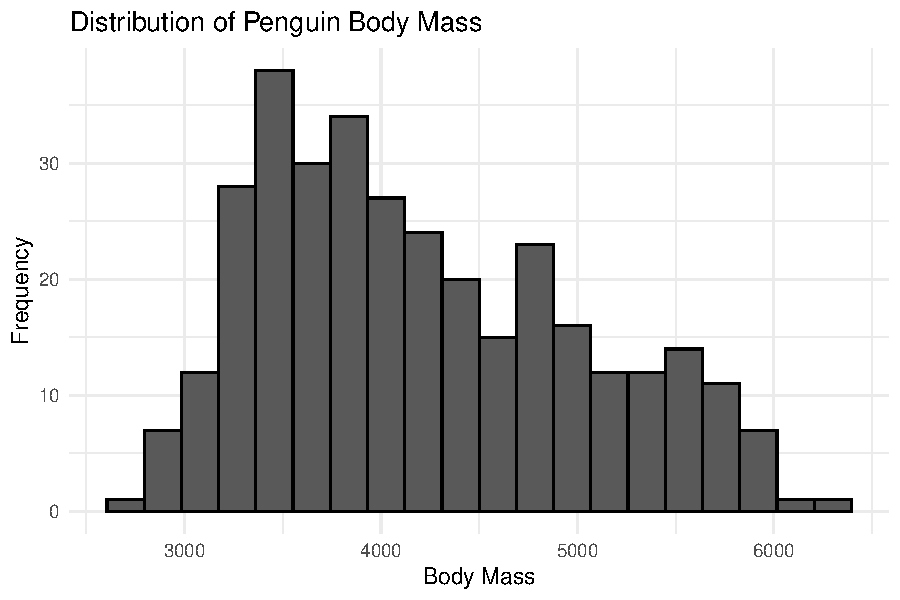
\includegraphics[width=0.9\linewidth]{main_files/figure-latex/data-hist-1} \end{center}

The histogram shows that penguin body masses range from approximately
2700 g to 6300 g, with most observations concentrated between 3000 g and
5000 g. The distribution shows a mild right skew, with a longer tail
toward higher body masses. This is consistent with the mean body mass
(4207.06 g) being higher than the median (4050 g). The distribution also
shows relatively high frequencies around 3500 to 4000 g, while fewer
observations are found at the upper end of the body mass range.

\subparagraph{Box Plot}\label{box-plot}

\begin{center}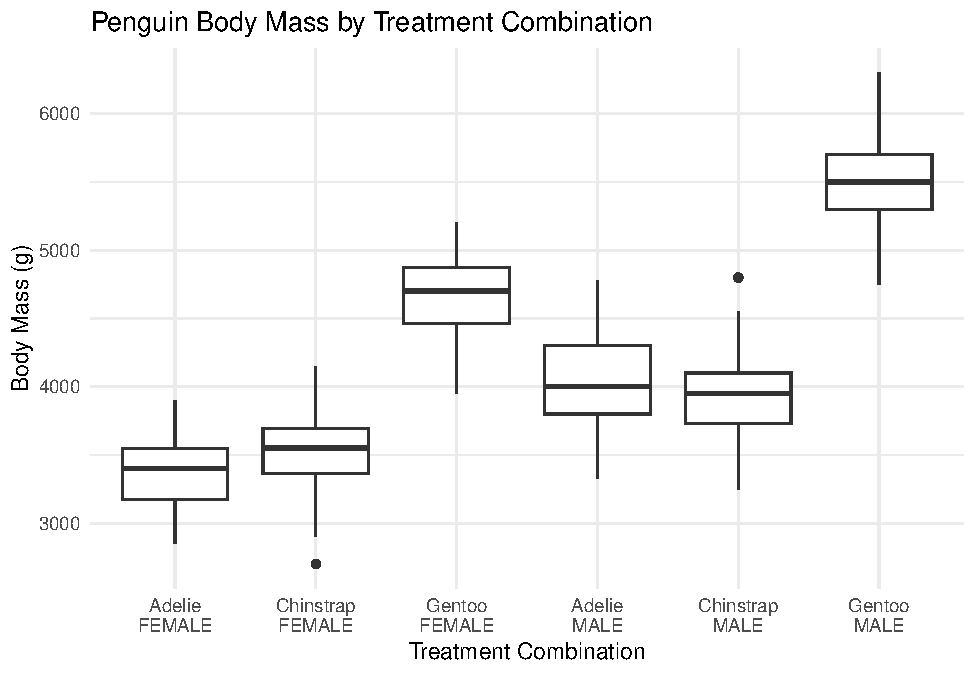
\includegraphics[width=0.95\linewidth]{main_files/figure-latex/data-boxplot-1} \end{center}

The box plot compares the distribution of penguin body mass across the
six treatment combinations of species and sex. Male penguins generally
have higher median and mean body mass than female penguins within each
species.

The difference between male and female body mass appears across all
three species. The largest difference is observed for Adelie penguins,
with mean body mass increasing from 3368.84 g for females to 4043.49 g
for males. For Chinstrap penguins, the corresponding means are 3527.21 g
and 3938.97 g, while for Gentoo penguins they are 4679.74 g and 5484.84
g.

The spread of the groups is not completely uniform, with some groups
showing wider variability than others. A few potential low outliers are
also visible, particularly in the Chinstrap female group. Overall, the
plot suggests that both species and sex may be associated with penguin
body mass, while the differences in the male-female effect across
species provide descriptive evidence of a possible interaction between
the two factors.

\subparagraph{Interaction Plot}\label{interaction-plot}

\begin{center}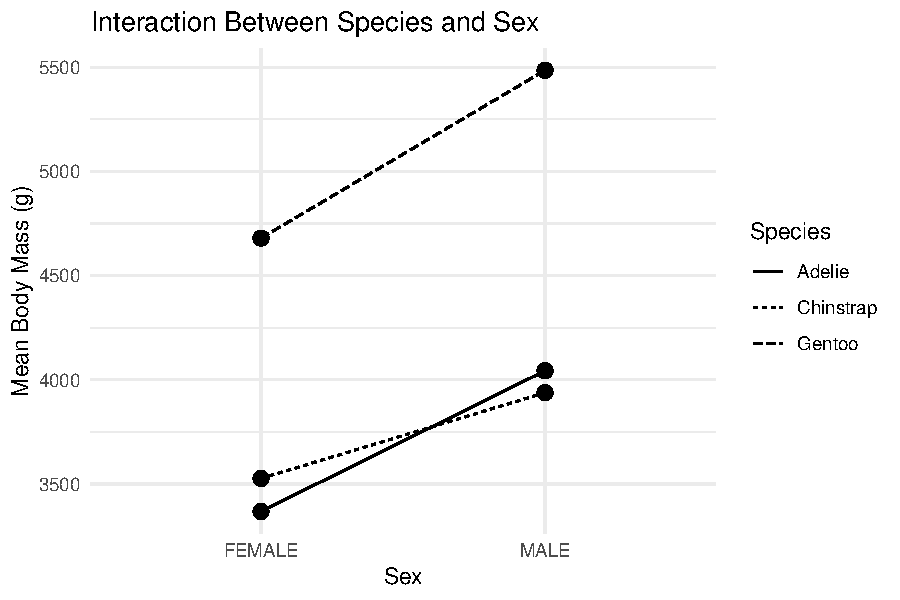
\includegraphics[width=0.9\linewidth]{main_files/figure-latex/interaction-plot-1} \end{center}

The interaction plot shows the mean body mass for each combination of
species and sex. Across all three species, male penguins have higher
mean body mass than female penguins. The mean body mass increases by
approximately 674.66 g for Adelie, 411.76 g for Chinstrap, and 805.10 g
for Gentoo penguins.

The lines are not perfectly parallel. In particular, the Adelie and
Chinstrap lines cross between the female and male groups, while the
Adelie and Gentoo lines show relatively similar slopes. This provides
some descriptive evidence that the difference in body mass between males
and females may vary across species.

However, the interaction pattern appears relatively modest overall, and
the plot alone cannot determine whether the interaction is statistically
significant. The significance of the species-by-sex interaction will be
formally assessed using the two-way ANOVA.

\paragraph{Assumptions Check}\label{assumptions-check}

\subparagraph{Normality of Residuals}\label{normality-of-residuals}

\begin{Shaded}
\begin{Highlighting}[]
\FunctionTok{shapiro.test}\NormalTok{(residual)}
\end{Highlighting}
\end{Shaded}

\begin{verbatim}
## 
##  Shapiro-Wilk normality test
## 
## data:  residual
## W = 0.99776, p-value = 0.9367
\end{verbatim}

The normality assumption was assessed using the Shapiro-Wilk test. The
hypotheses for the Shapiro-Wilk test are:

\[
\begin{cases}
H_0: \text{The residuals follow a normal distribution}\\
H_1: \text{The residuals do not follow a normal distribution}
\end{cases}
\]

The Shapiro-Wilk test resulted in

\[
W = 0.99776,\qquad p = 0.9367.
\]

Since the p-value is greater than 0.05, we fail to reject \(H_0\).
Therefore, there is no statistical evidence that the ANOVA residuals
deviate from a normal distribution. The Shapiro-Wilk test gives
\(W=0.99776\) with a p-value of \(0.9367\), providing further support
for the normality assumption.

Overall, the residuals show no substantial departure from normality, and
the normality assumption is considered satisfied for the subsequent
two-way ANOVA.

\subparagraph{Homogeneity of Variances}\label{homogeneity-of-variances}

\begin{Shaded}
\begin{Highlighting}[]
\FunctionTok{leveneTest}\NormalTok{(}
\NormalTok{  body\_mass\_g }\SpecialCharTok{\textasciitilde{}}
\NormalTok{    species }\SpecialCharTok{*}\NormalTok{ sex,}
  \AttributeTok{data =}\NormalTok{ analysis\_data}
\NormalTok{)}
\end{Highlighting}
\end{Shaded}

\begin{verbatim}
## Levene's Test for Homogeneity of Variance (center = median)
##        Df F value Pr(>F)
## group   5  1.3908 0.2272
##       327
\end{verbatim}

The homogeneity of variance assumption was assessed using the treatment
group box plots and Levene's test. The six treatment combinations are
formed by \texttt{species} and \texttt{sex}.

The hypotheses are:

\[
\begin{cases}
H_0:
\sigma_1^2 = \sigma_2^2 = \sigma_3^2 = \cdots =\sigma_6^2\\
H_1:
\text{At least one treatment group has a different variance}
\end{cases}
\]

Levene's test produced

\[
F(5,327) = 1.3908,\qquad p = 0.2272
\] Since the p-value is greater than 0.05, we fail to reject \(H_0\).
Therefore, there is no statistical evidence that the variances differ
across the six treatment combinations.

The group variances range from approximately 72,565.64 to 120,278.25,
with the Adelie male group having the largest variance and the Adelie
female group having the smallest variance. Although the group variances
are not identical, Levene's test suggests that the differences are not
statistically significant. Therefore, the homogeneity of variance
assumption is considered satisfied for the subsequent two-way ANOVA.

\subparagraph{Independence of Errors}\label{independence-of-errors}

\begin{Shaded}
\begin{Highlighting}[]
\FunctionTok{sum}\NormalTok{(}\FunctionTok{duplicated}\NormalTok{(analysis\_data))}
\end{Highlighting}
\end{Shaded}

\begin{verbatim}
## [1] 169
\end{verbatim}

The independence assumption requires that the error terms are
independent:

\[
\epsilon_{ijk} \overset{ind}{\sim} N(0,\sigma^2).
\]

The independence assumption was assessed based on the structure of the
dataset. Each observation represents an individual penguin, and the
dataset does not contain repeated measurements or a time-dependent
structure. Although some observations have identical values for the
selected variables (\texttt{body\_mass\_g}, \texttt{species}, and
\texttt{sex}), these do not necessarily represent duplicate penguins,
since different penguins can naturally have the same body mass and
characteristics.

Therefore, independence is considered reasonable based on the available
dataset information. However, it cannot be formally verified because the
dataset does not provide a unique identifier or detailed information
about the sampling procedure.

\paragraph{Overall Assessment}\label{overall-assessment}

The independence assumption is considered reasonable based on the
structure of the dataset. Each observation represents an individual
penguin, and there is no time-dependent or repeated-measurement
structure identified in the analysis data. However, independence cannot
be formally verified because the dataset does not provide a unique
identifier or detailed information about the sampling procedure.

The normality assumption is considered satisfied based on both the Q-Q
plot and the Shapiro-Wilk test (\(p=0.9367\)), which provides no
statistical evidence of a departure from normality. The homogeneity of
variance assumption is also considered satisfied based on the
non-significant Levene's test (\(p=0.2272\)).

Overall, the assumptions are considered reasonably adequate for
conducting the two-way ANOVA. No substantial concerns are observed
regarding normality or homogeneity of variance, while the independence
assumption is considered reasonable based on the available dataset
information.

\subsection{ANOVA / Factorial design
analysis}\label{anova-factorial-design-analysis}

\begin{Shaded}
\begin{Highlighting}[]
\NormalTok{model }\OtherTok{\textless{}{-}} \FunctionTok{aov}\NormalTok{(body\_mass\_g }\SpecialCharTok{\textasciitilde{}}\NormalTok{ species }\SpecialCharTok{*}\NormalTok{ sex ,}\AttributeTok{data=}\NormalTok{analysis\_data)}
\end{Highlighting}
\end{Shaded}

\begin{longtable}[]{@{}lrrrrr@{}}
\caption{ANOVA result}\tabularnewline
\toprule\noalign{}
& Df & Sum Sq & Mean Sq & F value & Pr(\textgreater F) \\
\midrule\noalign{}
\endfirsthead
\toprule\noalign{}
& Df & Sum Sq & Mean Sq & F value & Pr(\textgreater F) \\
\midrule\noalign{}
\endhead
\bottomrule\noalign{}
\endlastfoot
species & 2 & 145190219 & 72595109.56 & 758.358 & 0 \\
sex & 1 & 37090262 & 37090261.78 & 387.460 & 0 \\
species:sex & 2 & 1676557 & 838278.37 & 8.757 & 0 \\
Residuals & 327 & 31302628 & 95726.69 & NA & NA \\
\end{longtable}

Using significant level \(\alpha\) of 0.05, we observe that all these
p-value are less than \(\alpha\).

For species, the sum of squares is 145,190,219, which is the largest
among all factors. Together with the very large F-value of 758.358 and p
\textless{} 0.001, this indicates that species explains a very large
amount of the variation in the response variable and has a highly
significant effect.

For sex, the sum of squares is 37,090,262, which is also large compared
with the residual sum of squares. The F-value of 387.460 and p
\textless{} 0.001 show that sex has a highly significant effect on the
response variable.

For the species - sex interaction, the degrees of freedom is 2, because
the interaction involves the three species and two sex groups. Its sum
of squares is 1,676,557, which is much smaller than the sums of squares
for species and sex. However, the interaction is still statistically
significant, with an F-value of 8.757 and p \textless{} 0.001. This
indicates that although the interaction explains less variation, the
effect of sex still differs significantly among species.

Overall, species contributes the largest amount of variation, as shown
by its highest Sum Sq (145,190,219) and F-value (758.358). Sex also
contributes a substantial amount of variation, with a Sum Sq of
37,090,262 and F-value of 387.460. The interaction has a much smaller
Sum Sq (1,676,557) and F-value (8.757), but it remains significant.
Therefore, all three effects---species, sex, and species x sex are
statistically significant (p \textless{} 0.001), with species showing
the strongest effect.

\pandocbounded{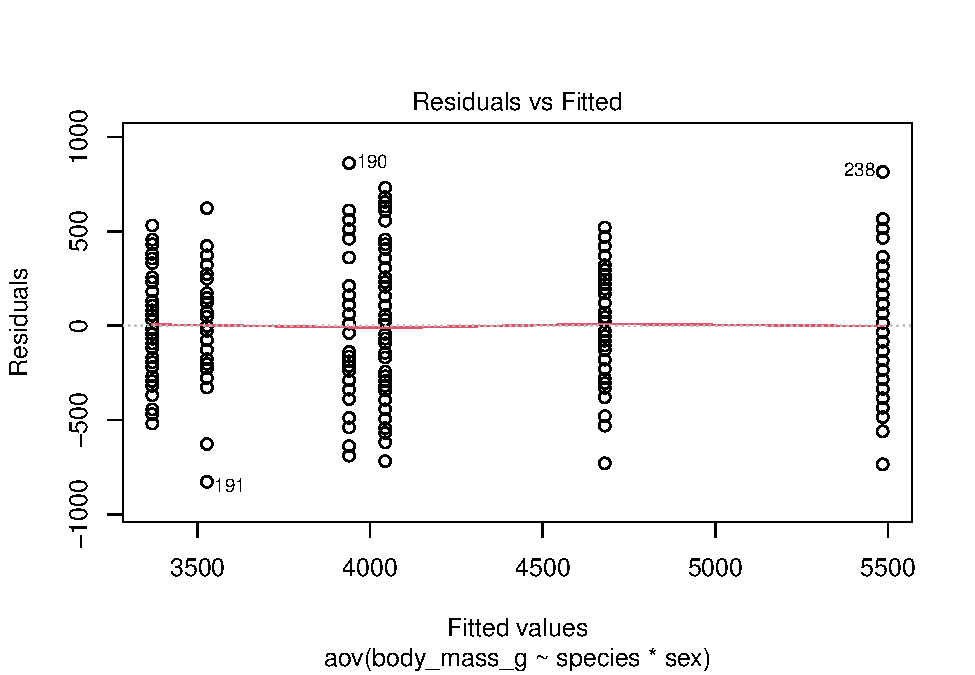
\includegraphics[keepaspectratio]{main_files/main_files/figure-latex/unnamed-chunk-15-1.pdf}}
This residuals are generally scattered around the horizontal zero line
across the different fitted values, and the red trend line remains close
to zero. This indicates that there is no strong systematic pattern or
curvature in the residuals, suggesting that the ANOVA model captures the
main structure of the data reasonably well.

The spread of the residuals is somewhat different between the
fitted-value groups, but there is no clear funnel-shaped pattern where
the spread consistently increases or decreases as the fitted values
increase. Therefore, there is no strong visual evidence of severe
heteroscedasticity from this plot.

\pandocbounded{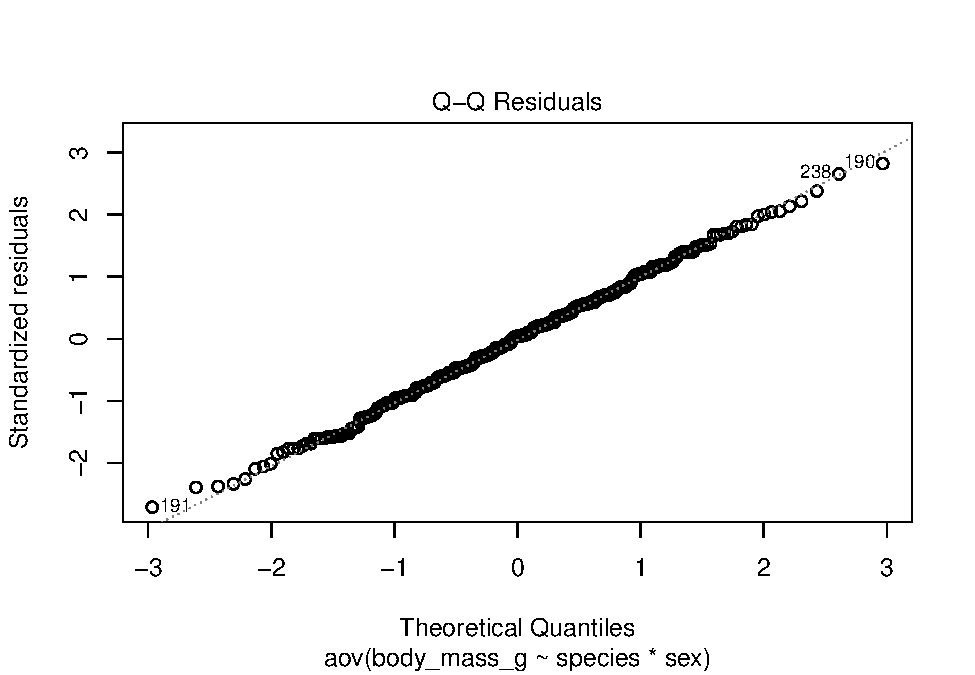
\includegraphics[keepaspectratio]{main_files/main_files/figure-latex/unnamed-chunk-16-1.pdf}}
This Q--Q plot shows most of the points closely follow the diagonal
reference line, particularly in the middle section of the plot,
indicating that the residuals are approximately normally distributed.
This suggests that the assumption of normality required for ANOVA is
reasonably satisfied.

\subsection{Posthoc analysis}\label{posthoc-analysis}

\begin{Shaded}
\begin{Highlighting}[]
\NormalTok{tukey }\OtherTok{\textless{}{-}} \FunctionTok{TukeyHSD}\NormalTok{(model, }\AttributeTok{which =} \StringTok{"species"}\NormalTok{)}
\end{Highlighting}
\end{Shaded}

\begin{longtable}[]{@{}lrrrr@{}}
\caption{Tukey HSD Results}\tabularnewline
\toprule\noalign{}
& diff & lwr & upr & p adj \\
\midrule\noalign{}
\endfirsthead
\toprule\noalign{}
& diff & lwr & upr & p adj \\
\midrule\noalign{}
\endhead
\bottomrule\noalign{}
\endlastfoot
Chinstrap-Adelie & 26.924 & -80.026 & 133.874 & 0.824 \\
Gentoo-Adelie & 1386.273 & 1296.307 & 1476.238 & 0.000 \\
Gentoo-Chinstrap & 1359.349 & 1248.611 & 1470.087 & 0.000 \\
\end{longtable}

The comparison between Chinstrap and Adelie is not statistically
significant, with an adjusted p-value of 0.824, which is greater than
0.05. The confidence interval also includes zero (-80.026 to 133.874).
Therefore, there is insufficient evidence to conclude that the mean
response differs between Chinstrap and Adelie.

In contrast, Gentoo differs significantly from Adelie, with a mean
difference of 1386.273 and an adjusted p-value less than 0.001. The 95\%
confidence interval (1296.307 to 1476.238) does not contain zero,
providing strong evidence that the two species have different mean
responses. Since the mean difference is positive, the mean response for
Gentoo is higher than Adelie by approximately 1386.273 units.

Similarly, Gentoo differs significantly from Chinstrap, with a mean
difference of 1359.349 and an adjusted p-value less than 0.001. The 95\%
confidence interval (1248.611 to 1470.087) is entirely positive,
indicating that the mean response for Gentoo is higher than Chinstrap by
approximately 1359.349 units.

Overall, the Tukey HSD results show that Gentoo is significantly
different from both Adelie and Chinstrap, whereas Adelie and Chinstrap
do not differ significantly from each other. This provides more specific
information about the significant species effect identified by the
ANOVA.

\begin{Shaded}
\begin{Highlighting}[]
\NormalTok{sex\_analysis }\OtherTok{\textless{}{-}} \FunctionTok{t.test}\NormalTok{(body\_mass\_g }\SpecialCharTok{\textasciitilde{}}\NormalTok{ sex,}\AttributeTok{data=}\NormalTok{analysis\_data)}

\NormalTok{tidy\_t\_test }\OtherTok{\textless{}{-}} \FunctionTok{tidy}\NormalTok{(sex\_analysis)}
\end{Highlighting}
\end{Shaded}

\begin{longtable}[]{@{}rrrrr@{}}
\caption{Independent t-test Comparing Penguin Body Mass by
Sex}\tabularnewline
\toprule\noalign{}
Mean Difference & t-Statistic & p-value & Lower CI & Upper CI \\
\midrule\noalign{}
\endfirsthead
\toprule\noalign{}
Mean Difference & t-Statistic & p-value & Lower CI & Upper CI \\
\midrule\noalign{}
\endhead
\bottomrule\noalign{}
\endlastfoot
-683.412 & -8.555 & 0 & -840.578 & -526.245 \\
\end{longtable}

An independent-samples t-test was conducted to compare penguin body mass
between male and female penguins. The results showed a mean difference
of -683.412 grams, with a t-statistic of -8.555 and a p-value of
\textless{} 0.001.

The very small p-value indicates a statistically significant difference
in body mass between the two sexes. The mean difference of -683.412
grams indicates that the first sex group in the comparison has an
average body mass approximately 683.4 grams lower than the second sex
group.

The 95\% confidence interval for the mean difference ranges from
-840.578 to -526.245 grams. Since the entire interval is below zero, the
estimated difference is consistently in the same direction. Therefore,
the results indicate that one sex has substantially greater average body
mass than the other.

Overall, sex is associated with a significant difference in penguin body
mass, with an average difference of approximately 683 grams between the
two sexes.

\begin{Shaded}
\begin{Highlighting}[]
\NormalTok{emm\_result }\OtherTok{\textless{}{-}} \FunctionTok{emmeans}\NormalTok{(model, pairwise }\SpecialCharTok{\textasciitilde{}}\NormalTok{ sex }\SpecialCharTok{|}\NormalTok{ species, }\AttributeTok{adjust =} \StringTok{"tukey"}\NormalTok{)}
\end{Highlighting}
\end{Shaded}

\begin{longtable}[]{@{}
  >{\raggedright\arraybackslash}p{(\linewidth - 12\tabcolsep) * \real{0.2000}}
  >{\raggedright\arraybackslash}p{(\linewidth - 12\tabcolsep) * \real{0.1429}}
  >{\raggedleft\arraybackslash}p{(\linewidth - 12\tabcolsep) * \real{0.2143}}
  >{\raggedleft\arraybackslash}p{(\linewidth - 12\tabcolsep) * \real{0.1571}}
  >{\raggedleft\arraybackslash}p{(\linewidth - 12\tabcolsep) * \real{0.0571}}
  >{\raggedleft\arraybackslash}p{(\linewidth - 12\tabcolsep) * \real{0.1143}}
  >{\raggedleft\arraybackslash}p{(\linewidth - 12\tabcolsep) * \real{0.1143}}@{}}
\caption{Pairwise Comparisons of Body Mass Between Sexes Stratified by
Penguin Species}\tabularnewline
\toprule\noalign{}
\begin{minipage}[b]{\linewidth}\raggedright
Contrast
\end{minipage} & \begin{minipage}[b]{\linewidth}\raggedright
Species
\end{minipage} & \begin{minipage}[b]{\linewidth}\raggedleft
Difference (g)
\end{minipage} & \begin{minipage}[b]{\linewidth}\raggedleft
Std. Error
\end{minipage} & \begin{minipage}[b]{\linewidth}\raggedleft
df
\end{minipage} & \begin{minipage}[b]{\linewidth}\raggedleft
t-ratio
\end{minipage} & \begin{minipage}[b]{\linewidth}\raggedleft
p.value
\end{minipage} \\
\midrule\noalign{}
\endfirsthead
\toprule\noalign{}
\begin{minipage}[b]{\linewidth}\raggedright
Contrast
\end{minipage} & \begin{minipage}[b]{\linewidth}\raggedright
Species
\end{minipage} & \begin{minipage}[b]{\linewidth}\raggedleft
Difference (g)
\end{minipage} & \begin{minipage}[b]{\linewidth}\raggedleft
Std. Error
\end{minipage} & \begin{minipage}[b]{\linewidth}\raggedleft
df
\end{minipage} & \begin{minipage}[b]{\linewidth}\raggedleft
t-ratio
\end{minipage} & \begin{minipage}[b]{\linewidth}\raggedleft
p.value
\end{minipage} \\
\midrule\noalign{}
\endhead
\bottomrule\noalign{}
\endlastfoot
FEMALE - MALE & Adelie & -674.658 & 51.212 & 327 & -13.174 & 0 \\
FEMALE - MALE & Chinstrap & -411.765 & 75.040 & 327 & -5.487 & 0 \\
FEMALE - MALE & Gentoo & -805.095 & 56.743 & 327 & -14.188 & 0 \\
\end{longtable}

Pairwise comparisons showed that male penguins had significantly higher
body mass than females in all three species (p\textless0.001). The
differences were approximately 674.7 g for Adelie, 411.8 g for
Chinstrap, and 805.1 g for Gentoo. The largest sex difference occurred
in Gentoo, while the smallest occurred in Chinstrap.

\subsubsection{Practical significance}\label{practical-significance}

The results are not only statistically significant but also practically
meaningful. The differences in body mass between species are large,
particularly between Gentoo and the other two species, with differences
of more than 1,300 g. The sex differences are also substantial, ranging
from approximately 412 g to 805 g, with males consistently heavier than
females.

Therefore, species and sex should be considered when assessing or
comparing penguin body mass. Ignoring these factors could lead to
misleading comparisons, especially when comparing groups with different
species or sex compositions.

\subsection{Conclusion and evaluation}\label{conclusion-and-evaluation}

The two-way ANOVA showed that species and sex both have significant
effects on penguin body mass (p\textless0.001). The Species x Sex
interaction was also significant (p\textless0.001), indicating that the
effect of sex on body mass varies among species. Tukey's HSD showed that
Gentoo differs significantly from both Adelie and Chinstrap, while
Adelie and Chinstrap do not differ significantly. Pairwise comparisons
further showed that males have significantly higher body mass than
females in all three species, with the largest difference observed in
Gentoo.

The analysis provides strong evidence of differences in body mass by
species and sex. However, the ANOVA assumptions should be considered,
particularly normality and homogeneity of variance. The data may also be
unbalanced across groups, which can affect the analysis. Future analysis
could use robust methods or transformations if assumption violations are
substantial.

Based on these results, species and sex should both be considered when
analyzing or predicting penguin body mass. In particular, the
significant interaction suggests that the effect of sex should not be
interpreted independently of species. Further studies could collect more
balanced samples across species and sexes to improve the reliability and
generalizability of the findings.

\end{document}
